%%%%%%%%%%%%%%%%%%%%%%% file template.tex %%%%%%%%%%%%%%%%%%%%%%%%%
%
% This is a general template file for the LaTeX package SVJour3
% for Springer journals.          Springer Heidelberg 2010/09/16
%
% Copy it to a new file with a new name and use it as the basis
% for your article. Delete % signs as needed.
%
% This template includes a few options for different layouts and
% content for various journals. Please consult a previous issue of
% your journal as needed.
%
%%%%%%%%%%%%%%%%%%%%%%%%%%%%%%%%%%%%%%%%%%%%%%%%%%%%%%%%%%%%%%%%%%%
%
% First comes an example EPS file -- just ignore it and
% proceed on the \documentclass line
% your LaTeX will extract the file if required
\begin{filecontents*}{example.eps}
%!PS-Adobe-3.0 EPSF-3.0
%%BoundingBox: 19 19 221 221
%%CreationDate: Mon Sep 29 1997
%%Creator: programmed by hand (JK)
%%EndComments
gsave
newpath
  20 20 moveto
  20 220 lineto
  220 220 lineto
  220 20 lineto
closepath
2 setlinewidth
gsave
  .4 setgray fill
grestore
stroke
grestore
\end{filecontents*}
%
\RequirePackage{fix-cm}
%
%\documentclass{svjour3}                     % onecolumn (standard format)
%\documentclass[smallcondensed]{svjour3}     % onecolumn (ditto)
\documentclass[smallextended]{svjour3}       % onecolumn (second format)
%\documentclass[twocolumn]{svjour3}          % twocolumn
%
\smartqed  % flush right qed marks, e.g. at end of proof
%
\usepackage{graphicx}
\usepackage{amsmath}
\usepackage{graphicx}
\usepackage{amssymb}

\usepackage{CJK}
\usepackage[top=2cm, bottom=2cm, left=2cm, right=2cm]{geometry}
\usepackage{algorithm}
\usepackage{algorithmicx}
\usepackage{algpseudocode}

\usepackage{multirow}
\usepackage{longtable}
\usepackage{footnote}

\floatname{algorithm}{algorithm}
\renewcommand{\algorithmicrequire}{\textbf{Input:}}
\renewcommand{\algorithmicensure}{\textbf{Output:}}
\usepackage{caption}

\usepackage[misc]{ifsym}
 \usepackage[numbers]{natbib}
 
\usepackage{array}
\usepackage{supertabular}
\makeatletter
\newenvironment{breakablealgorithm}
{% \begin{breakablealgorithm}
	\begin{center}
		\refstepcounter{algorithm}% New algorithm
		\hrule height.8pt depth0pt \kern2pt% \@fs@pre for \@fs@ruled
		\renewcommand{\caption}[2][\relax]{% Make a new \caption
			{\raggedright\textbf{\ALG@name~\thealgorithm} ##2\par}%
			\ifx\relax##1\relax % #1 is \relax
			\addcontentsline{loa}{algorithm}{\protect\numberline{\thealgorithm}##2}%
			\else % #1 is not \relax
			\addcontentsline{loa}{algorithm}{\protect\numberline{\thealgorithm}##1}%
			\fi
			\kern2pt\hrule\kern2pt
		}
	}{% \end{breakablealgorithm}
	\kern2pt\hrule\relax% \@fs@post for \@fs@ruled
\end{center}
}
\makeatother


%
% \usepackage{mathptmx}      % use Times fonts if available on your TeX system
%
% insert here the call for the packages your document requires
%\usepackage{latexsym}
% etc.
%
% please place your own definitions here and don't use \def but
% \newcommand{}{}
%
% Insert the name of "your journal" with
% \journalname{myjournal}

\begin{document}

\title{Synthesis of ranking functions via DNN%\thanks{Grants or other notes
%about the article that should go on the front page should be
%placed here. General acknowledgments should be placed at the end of the article.}
}
%\subtitle{Do you have a subtitle?\\ If so, write it here}

%\titlerunning{Short form of title}        % if too long for running head

\author{Wang Tan \textsuperscript{1,2}     \and
	Yi Li  \textsuperscript{2} 
}

\institute{
	\Letter Yi Li\\
	\email{liyi@cigit.ac.cn}\\       
	\at
	{1} University of Chinese Academy of Sciences, Beijing, 100049, China.
	\at
	{2} Chongqing Key Laboratory of Automated Reasoning and Cognition, Automated Reasoning and Cognition     Center,Chongqing Institute of Green and Intelligent Technology, Chinese Academy of Sciences, Chongqing, 400714, China.
}

%\authorrunning{Short form of author list} % if too long for running head


%\date{Received: date / Accepted: date}
% The correct dates will be entered by the editor


\maketitle

\begin{abstract}
We propose a new approach to synthesis of non-polynomial ranking functions for loops via deep neural network(DNN). Firstly, we construct a ranking function template by DNN structure. And then the coefficients of the template can be learned by the train-set we construct to get a candidate ranking function. Finally, the candidate ranking function  will be verified to show if it is a real ranking function. The experimental results show us that for some of loops from other work, we can find their ranking functions efficiently. Moreover, for some loops having multi-phase ranking functions obtained by existing methods, our method can directly detect their global ranking functions. Especially, our method can also detect the global ranking functions for some loops with transcendental terms.
\keywords{Ranking function \and DNN \and Termination \and Loop programs}
% \PACS{PACS code1 \and PACS code2 \and more}
% \subclass{MSC code1 \and MSC code2 \and more}
\end{abstract}

\section{Introduction}
\label{intro}
The analysis and verification of the termination of loop programs has become a hot topic in the field of computer programming research, and has attracted the attention of many scholars at home and abroad\cite{cousot2012abstract}\cite{10.1145/373243.360210}\cite{urban2013abstract}. However, the termination verification of program itself is a very difficult problem, which is undecidable\cite{braverman2006termination}\cite{turing1937on}\cite{10.1007/978-3-540-27813-9_6}. It is generally known that a standard method of proving loop termination is to find a ranking function. A function that can map a program state into an element of some well-founded ordered set, such that the value descends in the appropriate order whenever the loop completes an iteration, can be defined as a ranking function. Since descent in a well-founded set cannot be infinite, the existence of ranking functions implies the termination of loop programs.

Nowadays, there are some methods for synthesizing linear ranking functions and polynomial ranking functions. For loops with linear guards and linear updates, many methods\cite{colon2002practical}\cite{10.1007/978-3-540-24622-0_20}\cite{coloon2001synthesis}\cite{yuan2019detecting}\cite{li2019on} are established to generate their linear ranking functions. However, not all linear loops have a linear ranking function. Motivated by that, many researchers propose methods\cite{10.1145/2629488}\cite{bagnara2013eventual}\cite{bradley2005polyranking}\cite{ben2017multiphase}\cite{bradley2005linear}\cite{leike2014ranking}\cite{li2016depth} to combine multiple linear ranking functions to capture more complex patterns. For loops with polynomial guards and polynomial updates, \cite{chen2007discovering}\cite{cousot2005proving}\cite{shen2013generating}\cite{yuan2019ranking} develop some methods to generate polynomial ranking functions. Existing methods of synthesizing ranking functions usually predefine a linear or polynomial ranking functions template first. And then, different technologies such as linear programming(LP)\cite{colon2002practical}\cite{10.1007/978-3-540-24622-0_20}\cite{coloon2001synthesis}\cite{10.1145/2629488}, semidefinite programming (SDP)\cite{cousot2005proving}\cite{shen2013generating} or quantifier elimination (QE)\cite{chen2007discovering} are used to get the values of the parameters in the template. For instance, in \cite{chen2007discovering} the detection of polynomial ranking functions is reduced to the semi-algebraic systems solving. And in \cite{yuan2019ranking}, the synthesis of polynomial ranking functions is reduced to the classification problem, where candidate ranking functions are obtained by Support-Vector Machines (SVM)\cite{fan2008liblinear:}\cite{li2019synthesizing} and then certified by \emph{Z3}\cite{10.1007/978-3-540-78800-3_24}. Nevertheless, for some loops, their ranking functions may be non-polynomial, such as transcendental ranking functions. Unfortunately, if such case occurs, \emph{Z3} cannot verify if such a candidate ranking function containing transcendental terms is a real ranking function. Moreover, existing methods cannot deal with the loops containing transcendental terms.

In this paper, we propose a new approach to synthesize ranking functions via DNN, which extends the form of ranking functions from polynomial forms to non-polynomial forms. In other words, we obtain a candidate ranking function by DNN first, then verify if this function we gotten is a ranking function by a new method which is independent of Z3. It is easy to see that the ranking functions template defined by DNN is transcendental rather than polynomial. And the weights $w_{i}$ and $w_{ji}$ in such template can be regarded as the parameters. Thus, our goal is to obtain the values of the parameters $w_{i}$ and $w_{ji}$ by training.

The rest of this paper is structured as follows. Sect. \ref{Preliminaries} introduces some preliminaries on ranking functions and DNN. Sect. \ref{DNN-Based Synthesis of Ranking Functions} introduces our approach to the synthesis of ranking functions by DNN. Sect. \ref{Exact Verification} gives a new method to verify whether or not a candidate ranking function is a ranking function. Sect. \ref{Experiments} demonstrates experimental results. Sect. \ref{Conclusion} concludes.

\section{Preliminaries}
\label{Preliminaries}
In this section we will introduce some basic notions on loop programs, ranking functions, and deep neural network.
\subsection{Forms of loop programs}
\label{Forms of loop programs}
In this paper we mainly consider loops of the following forms:
\begin{equation}\label{equ:the form of loop}
\ while\mathop  \wedge \limits_{i = 1}^{\rm{m}} {g_i}(x) \le 0\,\,do\,\mathop  \wedge \limits_{i = 1}^n {x'_i} = {f_i}(x)\
\end{equation}
where $x = {({x_1},{x_2}, \cdots ,{x_n})^T} \in {R^n}$ is an n-dimensional vector of variables, the conjunction of inequalities $\mathop  \wedge \limits_{i = 1}^{\rm{m}} {g_i}(x) \le 0$ is guard condition over the variables, and $\,\mathop  \wedge \limits_{i = 1}^n {x'_i} = {f_i}(x)$ is called the deterministic update, which means that for a given ${x}$ satisfying the loop condition defined as above, there is only at most one ${x'}$ satisfying the update constraint $\mathop  \wedge \limits_{i = 1}^n {x'_i} = {f_i}(x)$, where ${x'_i}$ denotes the new value of ${x_i}$  after each loop iteration. Let $x' = {({x_1}^\prime ,{x_2}^\prime , \cdots ,{x_n}^\prime )^T}$ and $f(x) = ({f_1}(x),{f_2}(x), \cdots ,{f_n}(x))$. So, $x' = f(x)$. In this paper, we only focus on loops with deterministic updates defined as above. 

Let
\begin{equation}
\Omega  = \{ x \in {R^n}:\mathop  \wedge \limits_{i = 1}^{\rm{m}} {g_i}(x) \le 0\,\,\}.
\end{equation}

We take an example to illustrate the concepts mentioned above.

\newtheorem{exam}{Example}
\begin{exam}
	\label{exam1}
	Consider the following loop:
	
	$$\begin{array}{l}
	while\;\;{x_1}^2 + {x_2}^2 \le 1\quad do\\
	{{x_1}'} = {x_1} - {x_2}^2 + 1,{{x_2}'} = {x_2} + {x_1}^2 - 1
	\end{array}$$
	
	In this loop, the guard condition is the inequality ${x_1}^2 + {x_2}^2 \le 1$ and $\Omega  = \{({x_{\rm{1}}},{x_2})\in R^2:{x_1}^2\, + {x_2}^2\, \le 1\} $. The update is 
	${x'_1} = {x_1} - {x_2}^2 + 1,{x'_2} = {x_2} + {x_1}^2 - 1$
	
\end{exam}
\subsection{Ranking functions}
\label{Ranking functions}
A loop program is terminating over the reals, if it terminates on all initial values of $x$ over ${R^n}$ . It is well known that the termination of loops is undecidable. The dominant method to proving termination is to synthesize ranking functions, since the existence of ranking functions implies termination.
\newtheorem{mydef}{Definition}
\begin{mydef} \label{def}
	Given a loop program, let $\Omega$ be a set specified by its loop guards. A function $r(x)$: ${R^n} \to R$ is a ranking function for the loop, if the following two conditions are satisfied.
	\begin{flushleft}
		{\bfseries Bounded.} $\forall x \in \Omega  \to r(x)\,\, \ge \,\,{\rm{0}}$
		
		{\bfseries Decreasing.} $\forall x \in \Omega  \to r(x) - r(f(x)) \ge c^+$
	\end{flushleft}
\end{mydef}
Where $c^+ > 0$. The existence of a ranking function implies termination.
\subsection{Deep Neural Network}
\label{Deep Neural Network}
Neural network work with functionalities similar to human brain. Deep-learning methods are
representation-learning methods with multiple levels of representation. We can extract features from original data by simple but non-linear modules. As long as these modules are enough, even very complex models can be represented.\cite{lecun2015deep}. And in this work, the deep neural network (DNN) we used can extract features from the train-set and detect complicated ranking functions.

The universal approximation theorem\cite{hornik1989multilayer}\cite{hornik1990universal}\cite{leshno1993original} states that a feed-forward network with a single hidden layer containing a finite number of neurons can approximate continuous functions on compact subsets of $R$, under mild assumptions on the activation function. Therefore, we attempt to leverage the DNN techniques for training a ranking function for a loop program. 
\section{DNN-Based Synthesis of Ranking Functions}
\label{DNN-Based Synthesis of Ranking Functions}
There are many methods to synthesize ranking functions, most of which focus on linear ranking functions and polynomial ranking functions. But there are few researches on non-polynomial ranking functions\cite{li2019synthesizing}. In this paper, we take a further step and propose a new method to find non-polynomial ranking functions by neural network. 

In the section, we give a particular function $U(x)$ which maps $\Omega $ to $U(\Omega )$ firstly such that $U(\Omega)$ is bounded. Then, we build a neural network architecture and introduce a method to get sample points for constructing the train-set. we can leverage the train-set to detect a candidate ranking function by DNN finally.

The key step in our method is to get sample points. The existing sampling methods are random sampling, but when $U(\Omega)$ is not bounded, the sampling points may not be representative by random sampling. Therefore, we first introduce a function $U(x)$ to map $\Omega $ to the $U(\Omega )$, such that the image set $U(\Omega )$ is a bounded set. And then by Theorem \ref{thm1}, we reduce equivalently the synthesis problem of ranking functions over $\Omega $ to $U(\Omega )$. Since $U(\Omega )$ is bounded, we can construct the sample points set, such that the union of neighborhoods of all sample points covers $U(\Omega )$.

Let $U(x) = (m({x_1}),m({x_2}), \cdots m({x_n}))$ be a mapping from $\Omega $ to $U(\Omega )$, where $m({x_i}) = \frac{1}{{1 + {e^{ - {x_i}}}}}$ is a sigmoid function. Thus, we have the image set $U(\Omega )$ of $\Omega$,
\begin{equation}\label{equ:Ux}
U(\Omega ) = \{ ({u_1},{u_2}, \cdots ,{u_n}) \in {R^n}:\mathop  \wedge \limits_{i = 1}^n {u_i} = m({x_i}), for\;all\;({x_1},{x_2}, \cdots ,{x_n}) \in \Omega \}. 
\end{equation}

Since the sigmoid function $m({x_i})$ is bounded and continuous, $U(\Omega )$ is bounded. More importantly, since sigmoid function defined as ${u_i} = \frac{1}{{1 + {e^{ - {x_i}}}}}$ is invertible, which has inverse function ${x_i} = \ln (\frac{{{u_i}}}{{1 - {u_i}}})$, $U(\Omega )$ can be rewritten as:
\begin{equation}\label{equ:Uu}
U(\Omega ) = \{ ({u_1},{u_2}, \cdots ,{u_n}) \in {R^n}:\mathop  \wedge \limits_{i = 1}^{\rm{m}} {g_i}((\ln (\frac{{{u_1}}}{{1 - {u_1}}}),\ln (\frac{{{u_2}}}{{1 - {u_2}}}), \cdots ,\ln (\frac{{{u_n}}}{{1 - {u_n}}}))) \le 0\,\} \}. 
\end{equation}

It is easy to see that $U(\Omega) \subset (0,1)^n$, since the range of ${u_i} = \frac{1}{{1 + {e^{ - {x_i}}}}}$ is $(0,1)$.

Since ${u_i} = m({x_i})$, we have 
\begin{equation}\label{equ:u}
u = ({u_1},{u_2}, \cdots ,{u_n}) = (m({x_1}),m({x_2}), \cdots ,m({x_n})) = U(x)
\end{equation}
$m({x_i})$ is a sigmoid function, which is inverse function. 

Let ${{u_i}'} = m({{x_i}'})$, so ${{x_i}'} = {m^{ - 1}}({{u_i}'})$. 
Since ${x_i} = {m^{ - 1}}({u_i})$ and ${x'_i} = {m^{ - 1}}({u'_i})$, we have
\begin{equation}\label{equ:x}
x = ({x_1},{x_2}, \cdots ,{x_n}) = ({m^{ - 1}}({u_1}),{m^{ - 1}}({u_2}), \cdots ,{m^{ - 1}}({u_n})) = {U^{{\rm{ - 1}}}}(u)
\end{equation}
\begin{equation}\label{equ:x'}
x' = ({x'_1},{x'_2}, \cdots ,{x'_n}) = ({m^{ - 1}}({u'_1}),{m^{ - 1}}({u'_2}), \cdots ,{m^{ - 1}}({u'_n})) = {U^{{\rm{ - 1}}}}(u').
\end{equation}

Since ${{x_i}'} = {f_i}(x)$ and $x' = f(x)$, we have 
\begin{equation}\label{equ:u'}
u' = ({{u_1}'},{{u_2}'}, \cdots ,{{u_n}'}) = (m({{x_1}'}),m({{x_2}'}), \cdots ,m({{x_n}'}))=U(x') = U(f(x)) = U(f({U^{ - 1}}(u))).
\end{equation}

\begin{exam}\label{exam2}
	Consider further, the loop program defined by Example \ref{exam1}, we choose sigmoid function as component function of $U(x)$, i.e.,
	$$\begin{array}{l}
	{u_1} = m({x_1}) = \frac{1}{{1 + {e^{ - {x_1}}}}},{u_2} = m({x_2}) = \frac{1}{{1 + {e^{ - {x_2}}}}}\\
	({u_1},{u_2}) = (m({x_1}),m({x_2})) = (\frac{1}{{1 + {e^{ - {x_1}}}}},\frac{1}{{1 + {e^{ - {x_2}}}}})
	\end{array}$$
\end{exam}


\newtheorem{mythm}{Theorem}
\begin{mythm}\label{thm1}
	With the above notion, let $U(x)$ be defined as above. Then, there is a ranking function over $\Omega $ if and only if there is a ranking function over $U(\Omega )$.
\end{mythm}
\emph{proof.}
Assume $R(x)$ is a ranking function over $\Omega $. Then, $R(x)$ satisfies the following two conditions of ranking functions.

\emph{(a)} $\forall x \in \Omega  \Rightarrow R(x)\,\, \ge \,\,{\rm{0}}$ . 

\emph{(b)} $\forall x \in \Omega  \Rightarrow R(x) - R(f(x)) \ge c^+$, where $c^+$ is a positive number. 

Consider (a), since  $x = {U^{ - 1}}(u)$, we have 
\begin{equation}\label{equ:thm1(1)}
R({U^{ - 1}}(u))\,\, \ge \,\,{\rm{0}} \Rightarrow  R \circ {U^{ - 1}}(u)\, \ge \,\,{\rm{0}}, \;for\;all\;u \in U(\Omega).
\end{equation}

Consider (b), since $x=U^{-1}(u)$, we have 
\begin{equation}\label{equ:thm1(2)}
R({U^{ - 1}}(u)) - R(f({U^{ - 1}}(u))) \ge c^+ \Rightarrow R \circ {U^{ - 1}}(u) - R \circ f \circ {U^{ - 1}}(u) \ge c^+ \Rightarrow R \circ {U^{ - 1}}(u) - R \circ U^{-1} \circ U \circ f \circ {U^{ - 1}}(u) \ge c^+.
\end{equation}

Let $r = R \circ {U^{ - 1}}$, $\forall u \in U(\Omega )$, by (\ref{equ:u'}), we know $u'=U \circ f \circ {U^{ - 1}}(u)$. So, we have 
\begin{equation}\label{equ:thm1(3)}
R \circ {U^{ - 1}}(u) - R \circ U^{-1} \circ U \circ f \circ {U^{ - 1}}(u) \ge c^+ \Rightarrow R \circ {U^{ - 1}}(u) - R \circ U^{-1} (u') \ge c^+.
\end{equation}
Then, by (\ref{equ:thm1(1)}) and (\ref{equ:thm1(3)}), we get $r(u) \ge 0$ and $r(u)-r(u') \ge c^+$.

According to definition of ranking function, $r(u)$ is exactly a ranking function over $U(\Omega )$. Conversely, assume that $r(u)$ is a ranking function over $U(\Omega)$. Similar analysis can be applied to prove that there is a ranking function $R(x)$ over $\Omega$, since $u=U(x)$ and u is invertible. We omit the details here. $\square$

\newtheorem{rem}{Remark}
\begin{rem}
	If a given loop program has a ranking function $R(x)$ over $\Omega $, then we can find the corresponding ranking function $r(u)$ over the image set $U(\Omega )$ of $\Omega $, vice versa.
\end{rem}

Theorem \ref{thm1} enables us to reduce equivalently the synthesis problem of ranking functions over $\Omega $ to $U(\Omega )$. In another words, we just need to leverage DNN to detect ranking functions over $U(\Omega )$. To do this, firstly, we give the neural network structure and then, we construct train-set over $U(\Omega )$. We get a candidate ranking function by training finally.

\subsection{Model Building}
\label{Model Building}
The basic structure of neural network consists of input layer, hidden layer and output layer. It is noteworthy that different activation functions and different connection mode can be applied between adjacent network layers.

Since we need to construct ranking function template through neural network structure, in this paper, we choose full-connected.

The neural network model is related to the following terms:

\textbf{\emph{Neurons.}} In this paper, the inputs of neural network consists of sample points and bias terms, so the number of neurons in the input layer is $n+1$, where $n$ denotes the number of loop programs. Meanwhile, the number of the neuron in the output layer is one. Furthermore, the number of the neurons in the hidden layer can be adjusted in the experimental process. In our experiments, we usually set it to 3.

\textbf{\emph{Activation function.}} As seen from the above, in order to make a ranking function template satisfy the \textbf{\emph{bounded}} condition of ranking functions, the output layer should select a bounded function as its activation function. In our experiments, we set all activation functions in the neural network to be sigmoid functions.

\textbf{\emph{Layers.}} The ranking function template depends on the number of layers of neural network. Therefore, we can adjust different layers to obtain different training effects. In this paper, we use three-layer network structure.

To sum up, one can construct a ranking function template $r(u)$ over $U(\Omega )$ by the DNN structure shown in Figure \ref{neural structure}, which is as follows:

\begin{figure}
	% Use the relevant command to insert your figure file.
	% For example, with the graphicx package use
	\center{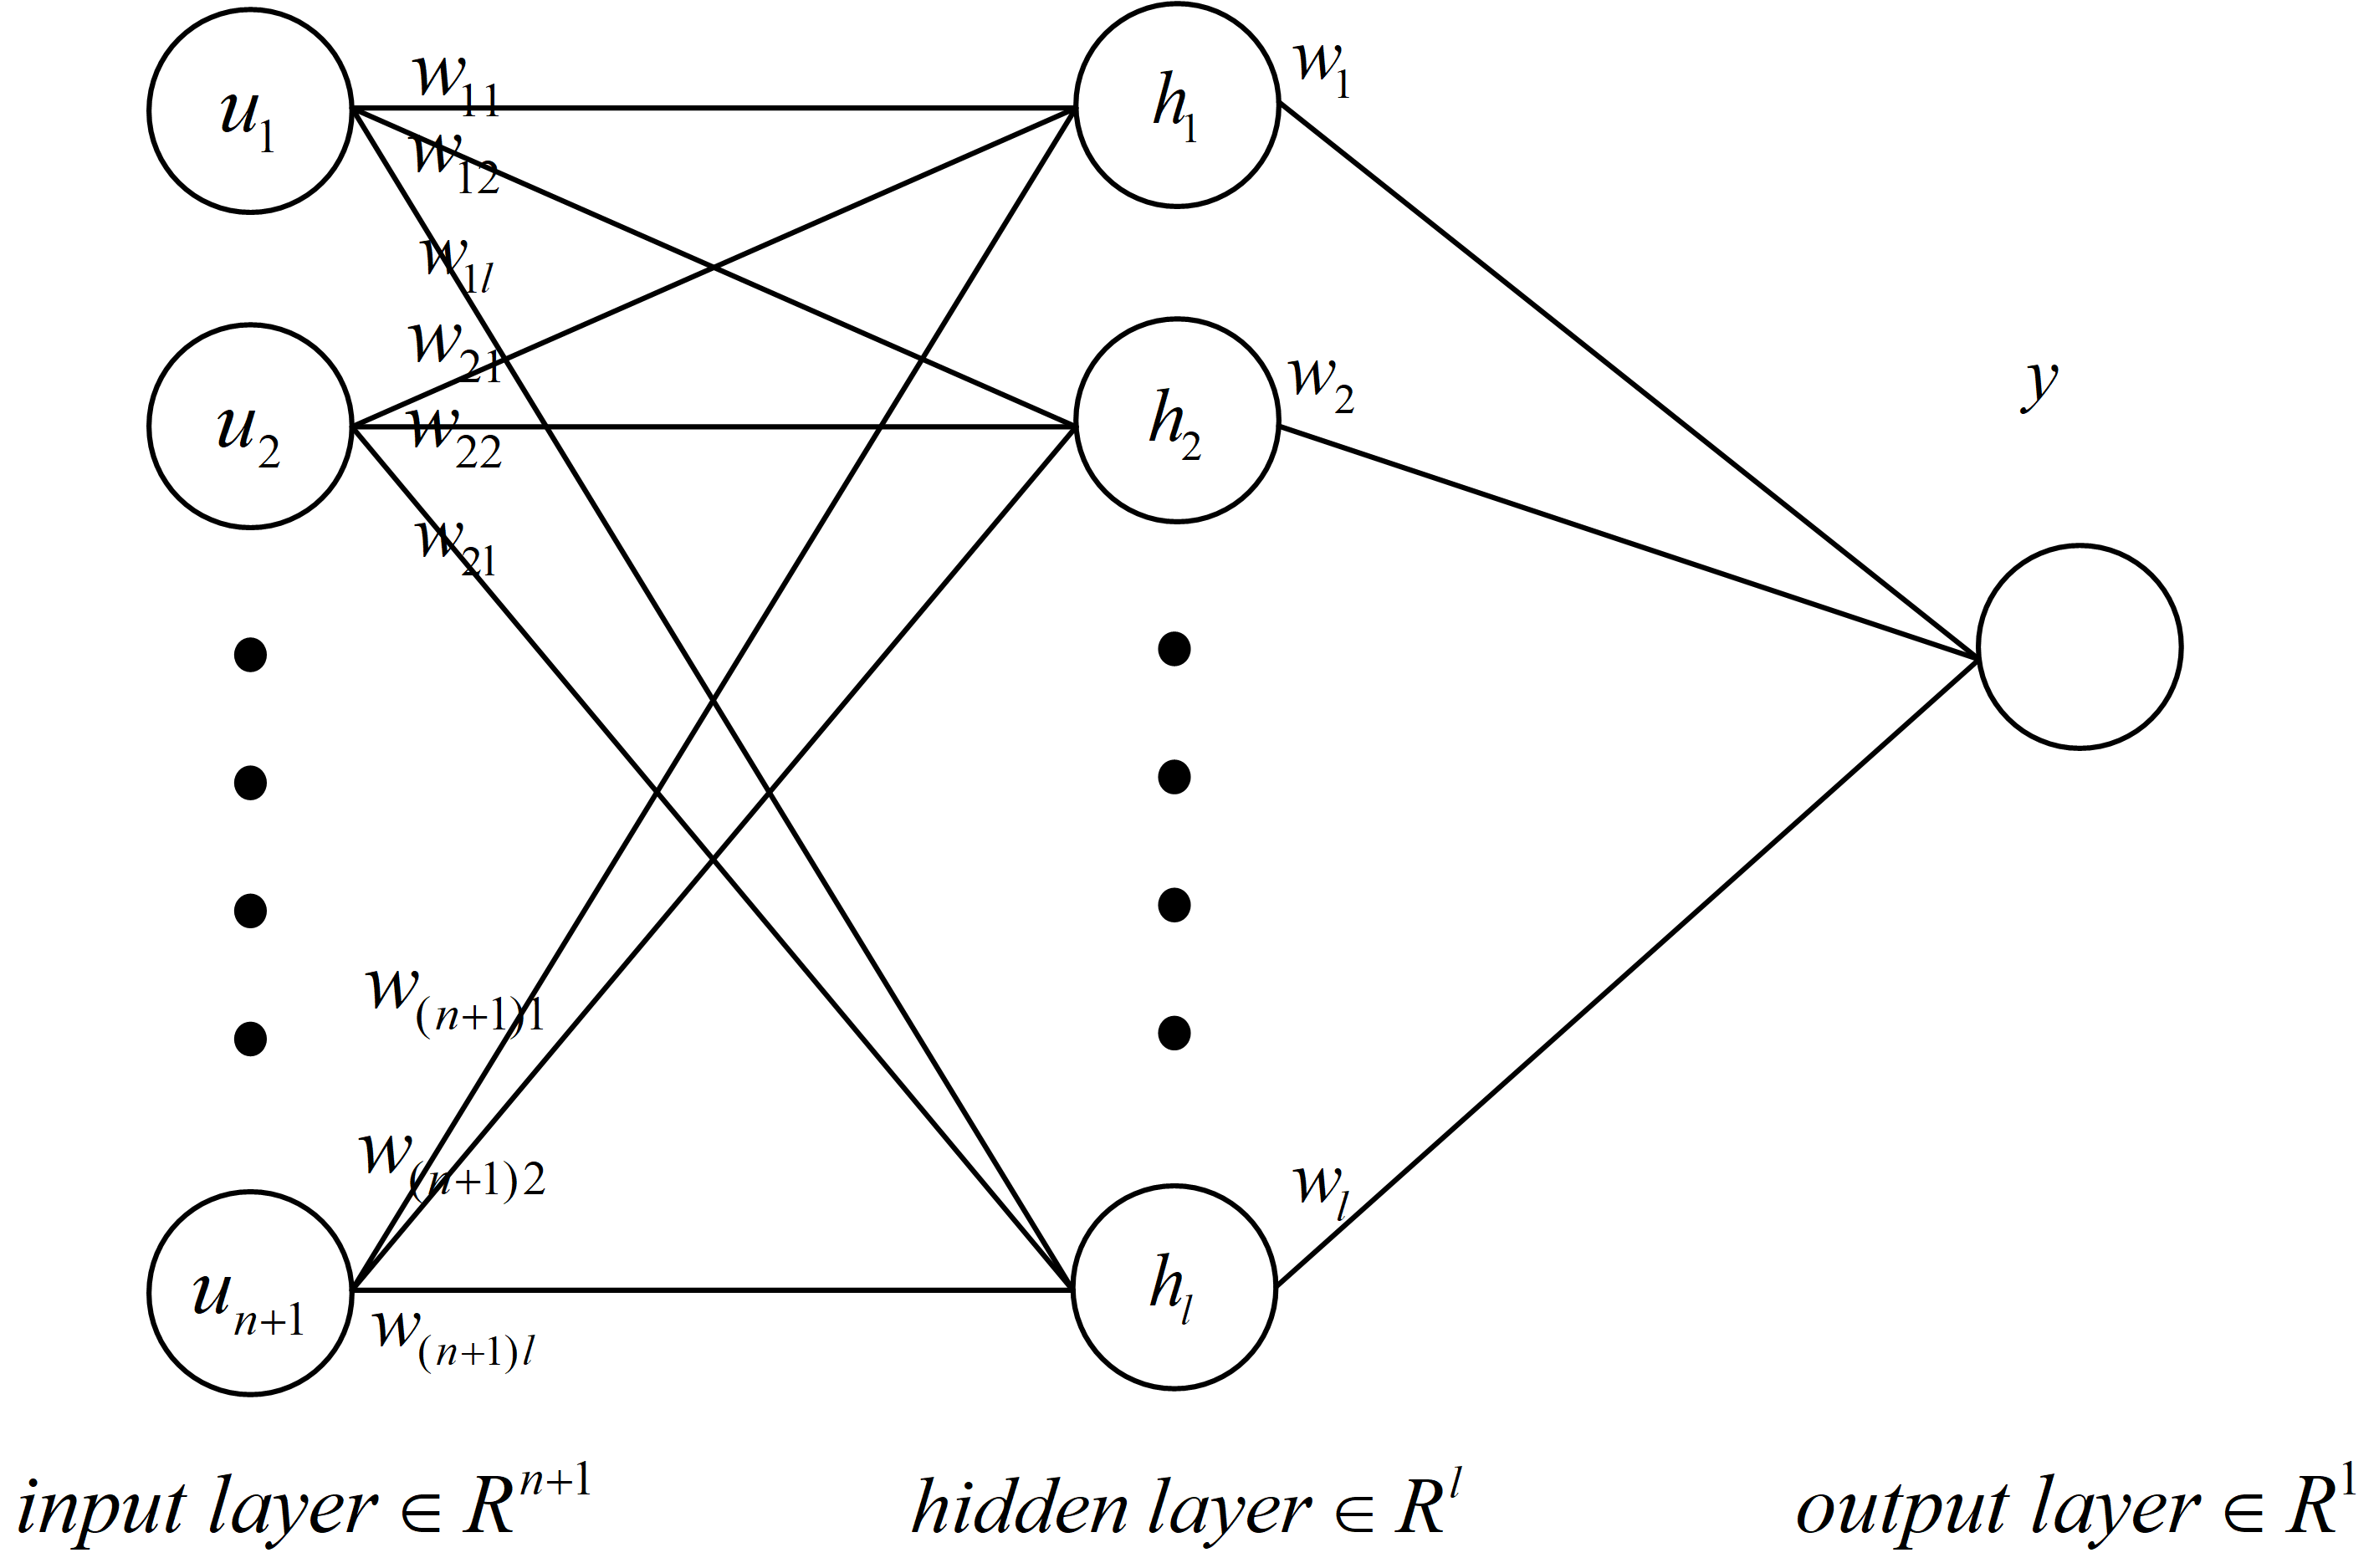
\includegraphics[width=10cm]  {1.png}} 
	% figure caption is below the figure
	\caption{Neural network structure}
	\label{neural structure}      % Give a unique label
\end{figure}
\begin{equation}\label{equ:r(u)}
r(u) = \frac{1}{{1 + {e^{ - (\sum\limits_{i = 1}^l {{w_i}\frac{1}{{1 + {e^{ - (\sum\limits_{j = 1}^{n{\rm{ + 1}}} {{w_{ji}}\cdot{u_j}} )}}}}} )}}}}.
\end{equation}

Note that $u = ({u_1},{u_2}, \cdots ,{u_{n + 1}})$, where ${u_{n + 1}} = 1$ is the bias term. In Figure \ref{neural structure}, $u_i$ is the input of neuron in the input layer and $h_i$ is the output of neuron in the hidden layer, while $y$ is the output of neuron in the output layer. ${w_i}$ is the weight for linking hidden layer and output layer. And ${w_{ji}}$ is the weight for linking hidden layer and input layer. Thus, finding a ranking function of loop programs is to derive the values of weights $w_i$ and $w_{ji}$ such that $r(u)$ satisfies the two conditions of ranking functions.
\subsection{Sample points set}
\label{Sample points set}
In this section, we will introduce how to construct sample points set. The following theorem tells us that $r(u)$ defined as in (\ref{equ:r(u)}) is bounded.

\begin{mythm}\label{thm2}
	With the above notion. Suppose the values of the parameters $w_i$ and $w_{ji}$ are given. Then, the function $r(u)$ must be bounded.
\end{mythm}
\emph{Proof.}
Suppose the output layer structure is shown in Figure \ref{outputlayer},
\begin{figure}[H] 
	% Use the relevant command to insert your figure file.
	% For example, with the graphicx package use
	\center{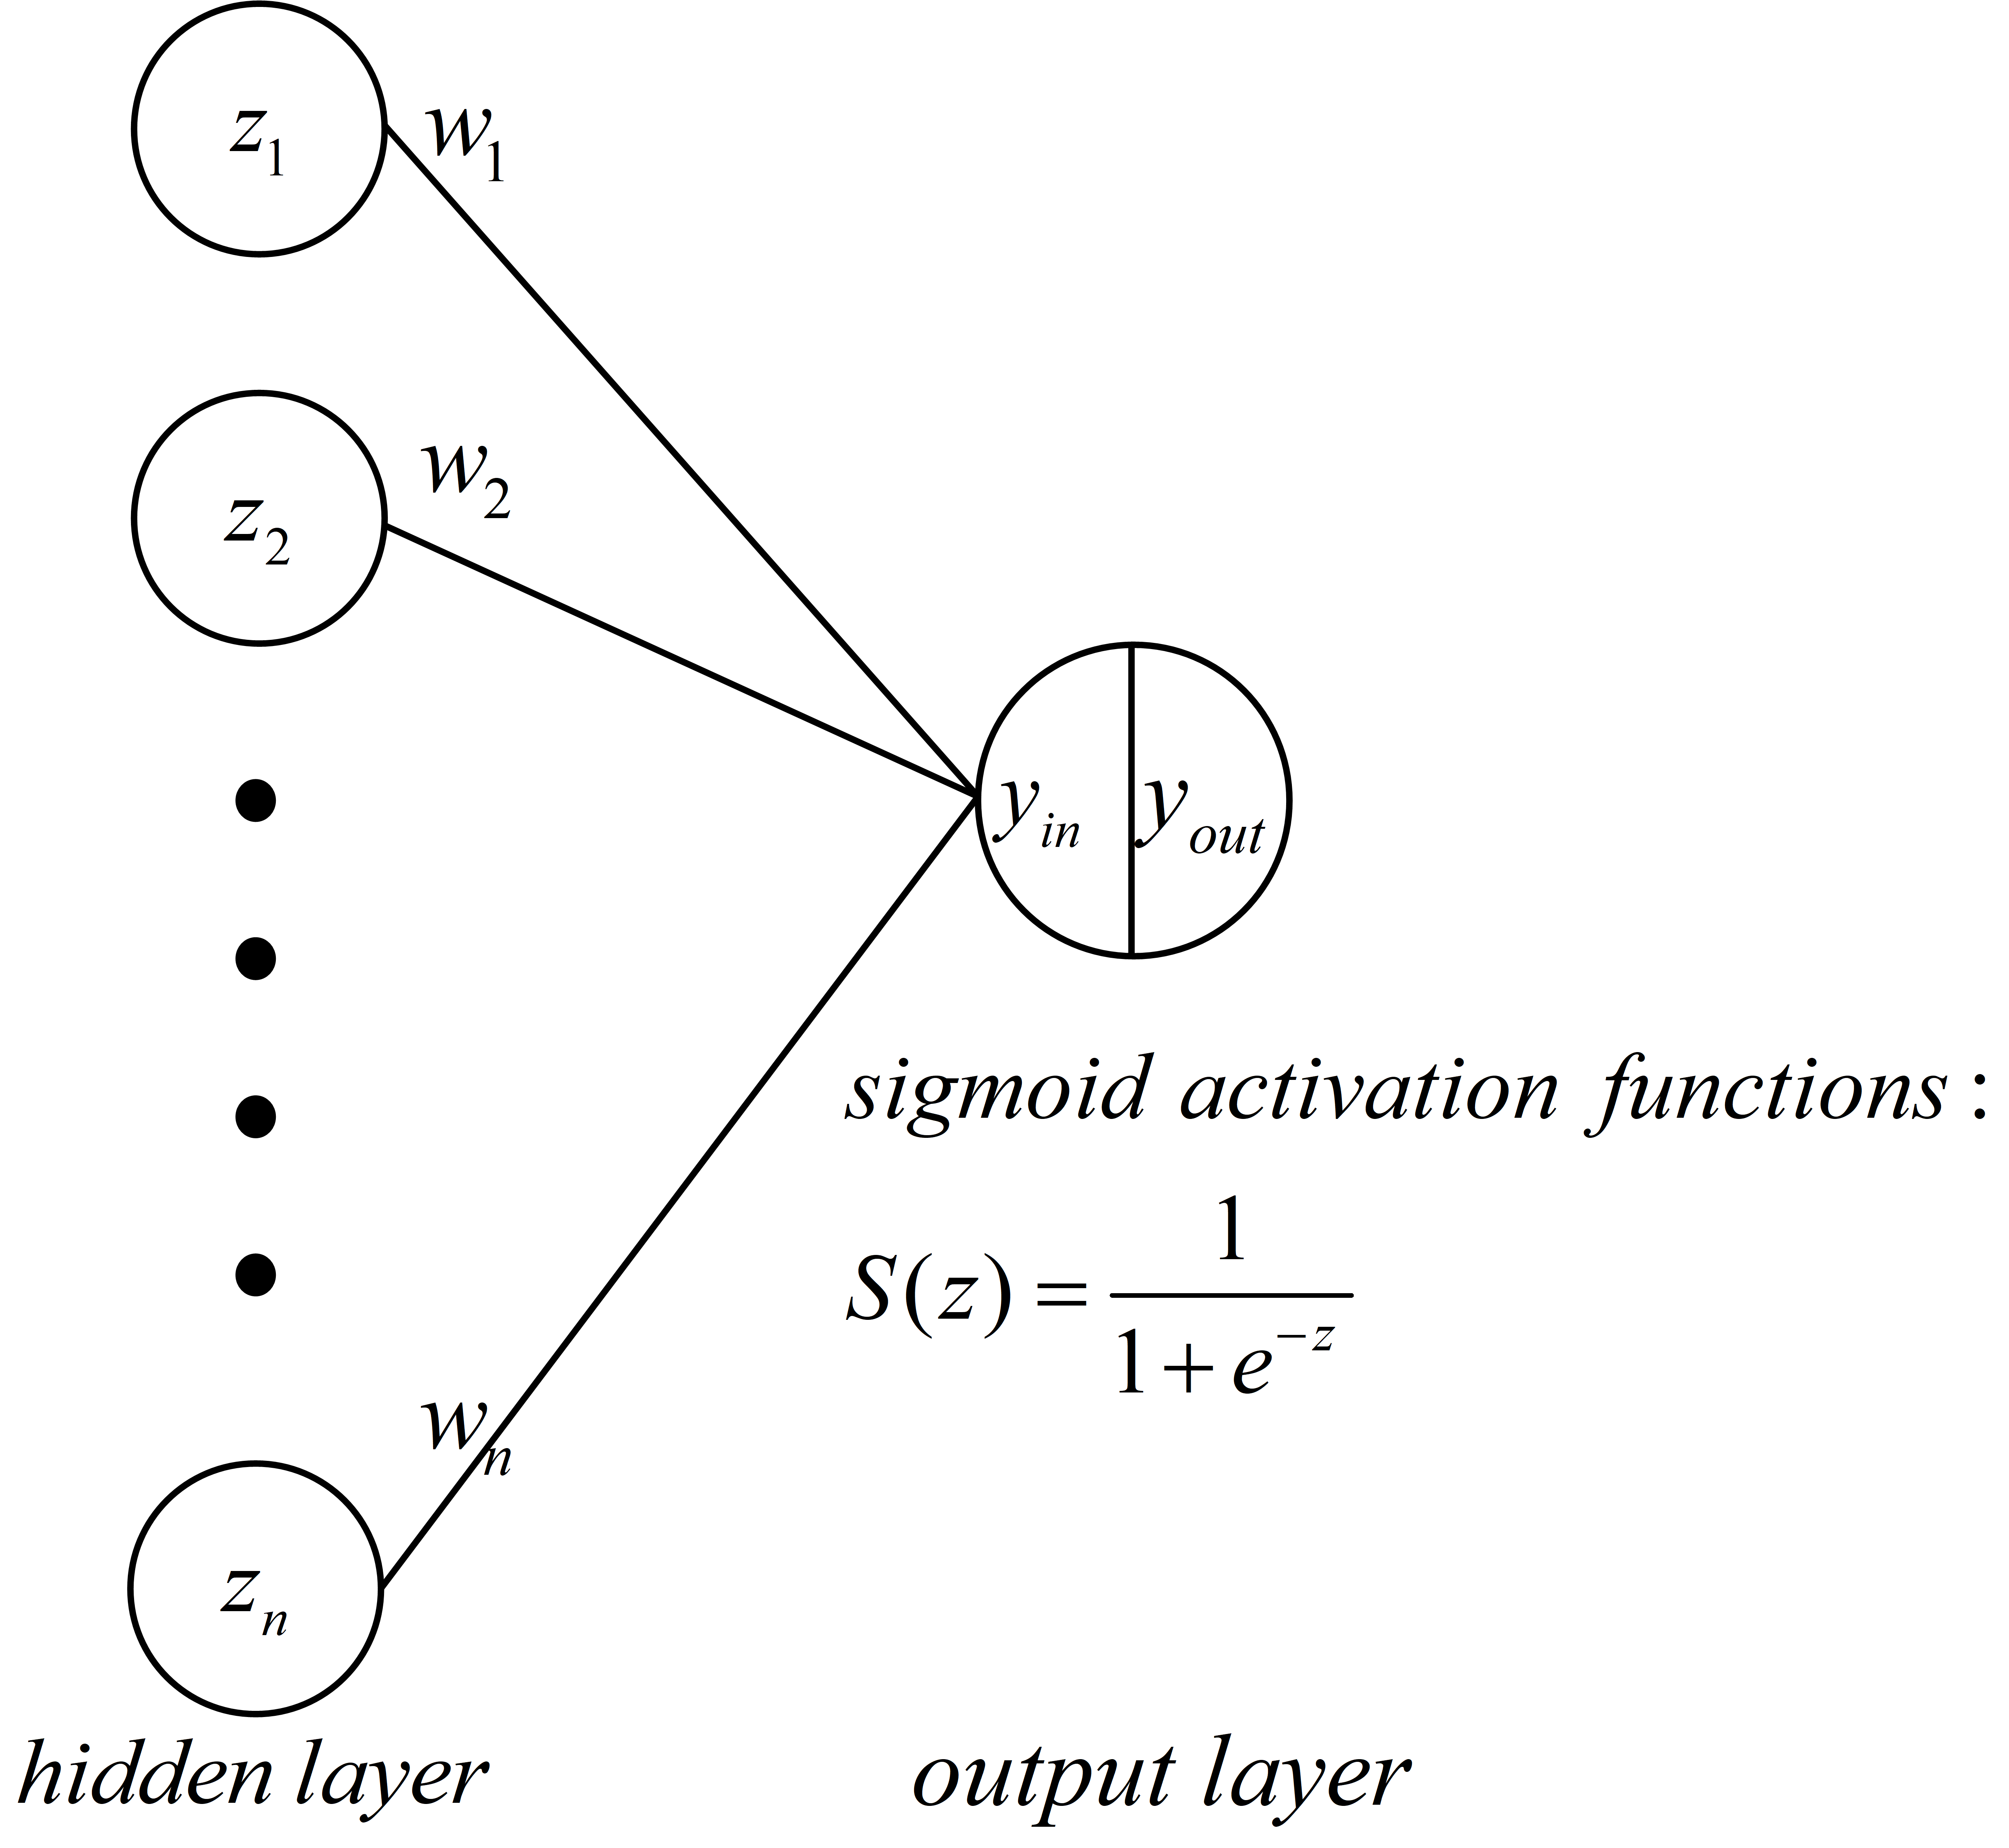
\includegraphics[width=5cm]  {2.png}} 
	% figure caption is below the figure
	\caption{Output layer structure}
	\label{outputlayer}      % Give a unique label
\end{figure}

Note that ${z_i},i \in (1,2, \cdots ,n)$ is the output of hidden layer, and ${w_i},i \in (1,2, \cdots ,n)$ is the weight. ${y_{in}}$ is the input of output layer, and ${y_{out}}$ is the output of output layer. ${y_{out}}$ can be calculated as follows:
\begin{equation}\label{equ:y}
\begin{array}{l}
{y_{in}} = \sum\limits_{i \in (1,n)} {{w_i}{z_i}} \\
{y_{out}} = \frac{1}{{1 + {e^{ - ({y_{in}})}}}}.
\end{array}
\end{equation}
It is easy to see that ${y_{in}}$ is the function of ${z_i}$, while ${y_{out}}$ is the function of ${y_{in}}$.
Owing to the range of the sigmoid function $S(z)=\frac{1}{{1 + {e^{ - z}}}}$ is $(0,1)$ for all $z \in (-\infty, +\infty)$. T hus ${y_{out}} \in (0,1)$, hence the function obtained by DNN must be bounded.$\square$

\begin{rem}
	Theorem \ref{thm2} tells us that the \textbf{\emph{bounded}} condition can be satisfied naturally when the activation function of output layer is a sigmoid function.
\end{rem}

In what follows, Owing to the \textbf{\emph{bounded}} condition is naturally satisfied by $r(u)$, we next just need to consider the \textbf{\emph{decreasing}} condition. That is, we want to obtain the value $w_i$ and $w_{ji}$, such that $\forall u \in U(\Omega ) \Rightarrow r(u) - r(u') \ge {c^ + }$ for a certain positive number $c^+$. Since $u' = U \circ f({U^{ - 1}}(u))$, the above formula can also be written as:
\begin{equation}\label{equ:decreasing condition}
\forall u \in U(\Omega ) \Rightarrow r(u) - r(U \circ f({U^{ - 1}}(u))) \ge {c^ + }.
\end{equation}

A natural technique is to use quantifier elimination (QE) to eliminate $u$ from (\ref{equ:decreasing condition}). However, since $r(u)$ is non-polynomial, QE-based technique cannot be applied to deal with (\ref{equ:decreasing condition}). Thus, in order to get the value of $w_i$ and $w_{ji}$ to guarantee that  $r(u) - r(U \circ f({U^{ - 1}}(u))) \ge {c^ + }$ holds on all $u$ in $U(\Omega)$, we propose a method to construct a finite points set $N_{sample}$ from $U(\Omega)$, such that $N_{sample}$ has the following properties:

\textbf{\emph{a.}} The union of neighborhoods of all points in $N_{sample}$ can cover $U(\Omega)$.

\textbf{\emph{b.}} For any a point $\alpha \in N_{sample}$, if $p(\alpha) \ge \varepsilon  > 0$, then for $\forall \theta \in {\rm O}(\alpha ,\delta )$, we have $p(\theta) \ge {c^ + }$, where ${\rm O}(\alpha ,\delta )$ is a neighborhood centered at $\alpha$ with radius $\delta$.

In the following, we will show how to construct $N_{sample}$. Since $U(\Omega ) \subseteq (0,1)^n$, we divide $(0,1)^n$ into a finite number of hypercubes with the same size $d$ by gridding technology. Here, how to choose step $d$ will be discussed in Theorem \ref{thm3}.

The following Theorem \ref{thm3} will show that under a certain condition, for given a point $\alpha $ in $N_{sample}$, if it satisfies $p(\alpha) \ge \varepsilon$, then for any point $\theta $ in its neighborhood ${\rm O}(\alpha ,\sqrt n d )$, we have $p(\theta) \ge \varepsilon-ndc$.

Let $\mathcal{H}$ be a convex set and $\Omega \subseteq \mathcal{H}$. Thus, clearly, the $\mathcal{U(H)}$ contains $U(\Omega)$, since $U(x)$ is invertible.
\begin{mythm}\label{thm3}
	Let $p(u) = r(u) - r(U \circ f({U^{ - 1}}(u)))$. Suppose that the upper bound in a hyperrectangle $\mathcal{U(H)}$ of $\left| \bigtriangledown p(u) \right|$ is $c$, for a given point $\alpha$, if $p(\alpha ) \ge \varepsilon  > 0$, then for $\forall \theta  \in {\rm O}(\alpha ,\sqrt n d )$ , we have $p(\theta ) \ge \varepsilon  - ndc$, where $p$ is a n-variate function, and ${\rm O}(\alpha ,\sqrt n d )$ is a neighborhood of radius $\sqrt n d$ with $\alpha $ as its center.
\end{mythm}
\emph{Proof.}
Let $\alpha  = ({\alpha _1},{\alpha _2}, \cdots ,{\alpha _n})$ and $\theta  = ({\theta _1},{\theta _2}, \cdots ,{\theta _n})$.

Suppose there is a point $\theta  \in {\rm O}(\alpha ,\sqrt n d )$, such that $p(\theta ) < \varepsilon  - ndc$.

Since $p(u)$ is continuous over $R^n$, according to the Lagrange mean value theorem, we get
\begin{equation}\label{equ:LMT}
p(\alpha ) - p(\theta ) = \bigtriangledown p(\beta ){\left( {{\alpha _1} - {\theta _1},{\alpha _2} - {\theta _2}, \cdots ,{\alpha _n} - {\theta _n}} \right)^T}
\end{equation}

where $\beta  = (\theta  + t\cdot(\alpha  - \theta )) \in \mathcal{U(H)},t \in (0,1)$.

Thus, by (\ref{equ:LMT}), we have
\begin{equation}\label{equ:|LMT|}
{\rm{|}}p(\alpha ) - p(\theta ){\rm{|}} = {\rm{|}}\bigtriangledown p(\beta ){\left( {{\alpha _1} - {\theta _1},{\alpha _2} - {\theta _2}, \cdots ,{\alpha _n} - {\theta _n}} \right)^T}{\rm{|}}.
\end{equation}

Since $p(\theta ) < \varepsilon  - ndc$ and $p(\alpha ) \ge \varepsilon $, it follows that 

\begin{equation}\label{equ:LMT(1)}
{\rm{|p(}}\alpha {\rm{) - p(}}\theta {\rm{)|}}\; \ge p(\alpha ) - p(\theta ) \ge \varepsilon  - p(\theta ) > \varepsilon  - (\varepsilon  - ndc) > ndc.
\end{equation} 

In addition, since
\begin{equation}\label{equ:LMT(b)}
{\rm{|}}\bigtriangledown p(\beta ){\left( {{\alpha _1} - {\theta _1},{\alpha _2} - {\theta _2}, \cdots ,{\alpha _n} - {\theta _n}} \right)^T}{\rm{|}}\; \le \;{\rm{|}}\bigtriangledown p(\beta ){\rm{|\cdot|}}{\left( {{\alpha _1} - {\theta _1},{\alpha _2} - {\theta _2}, \cdots ,{\alpha _n} - {\theta _n}} \right)^T}{\rm{|}}
\end{equation}

and
\begin{equation}\label{equ:LMT(b1)}
\begin{array}{l}
{\rm{|}}{\left( {{\alpha _1} - {\theta _1},{\alpha _2} - {\theta _2}, \cdots ,{\alpha _n} - {\theta _n}} \right)^T}{\rm{|}} = \sqrt {{{{\rm{(}}{\alpha _1} - {\theta _1}{\rm{)}}}^{\rm{2}}} + {{({\alpha _2} - {\theta _2})}^2} +  \cdots  + {{({\alpha _n} - {\theta _n})}^2}}  \\
\le \sqrt {{{{\rm{(}}\sqrt {\rm{n}} {\rm{d)}}}^{\rm{2}}} + {{(\sqrt {\rm{n}} {\rm{d}})}^2} +  \cdots  + {{(\sqrt {\rm{n}} {\rm{d}})}^2}}  = nd,
\end{array}
\end{equation}

we have
\begin{equation}\label{equ:LMT(2)}
{\rm{|}}\bigtriangledown p(\beta ){\left( {{\alpha _1} - {\theta _1},{\alpha _2} - {\theta _2}, \cdots ,{\alpha _n} - {\theta _n}} \right)^T}{\rm{|}}\; \le {\rm{ |\bigtriangledown p(}}\beta {\rm{)|}}\cdot nd.
\end{equation}

By (\ref{equ:|LMT|}), (\ref{equ:LMT(1)}) and (\ref{equ:LMT(2)}), since
\begin{equation}\label{equ:LMT(end)}
\begin{array}{l}
{\rm{|\bigtriangledown p(}}\beta {\rm{)|\cdot}}nd \ge {\rm{|}}\bigtriangledown p(\beta ){\left( {{\alpha _1} - {\theta _1},{\alpha _2} - {\theta _2}, \cdots ,{\alpha _n} - {\theta _n}} \right)^T}{\rm{|}}\;{\rm{ = {\rm{|}}p(}}\alpha {\rm{) - p(}}\theta {\rm{)|}}\; > ndc,
\end{array}
\end{equation}
we get
\begin{equation}\label{equ:contradicts}
{\rm{|\bigtriangledown p(}}\beta {\rm{)|}} > c.
\end{equation}
Clearly, (\ref{equ:contradicts}) contradicts the assumption ${\rm{|}}\bigtriangledown p(u)| \le c$ for all $u \in \mathcal{U(H)}$. 
Therefore, $\forall \theta  \in {\rm O}(\alpha ,\sqrt n d )$, we have $p(\theta ) \ge \varepsilon  - ndc$. $\square$

\begin{rem}
	Since $p = r(u) - r(U \circ f({U^{ - 1}}(u)))$, we can see that if ${\rm{|}}\bigtriangledown(r(u) - r(U \circ f({U^{ - 1}}(u))))|$ have a upper bound $c$ and a point $\alpha $ in $N_{sample}$ satisfy $r(\alpha) - r(U \circ f({U^{ - 1}}(\alpha))) \ge \varepsilon$, then for any point $\theta $ in the neighborhood ${\rm O}(\alpha ,\sqrt n d )$, we have $r(\theta) - r(U \circ f({U^{ - 1}}(\theta)))\ge \varepsilon-ndc$. 
\end{rem}

According to the \textbf{\emph{decreasing}} condition of ranking functions, which requires $p = r(u) - r(U \circ f({U^{ - 1}}(u))) \ge c^+$. We need to ensure that the $\varepsilon  - ndc$ is a positive number. Because $r(u)$ is a template with the parameters $w_i$ and $w_{ji}$, $c$ is a function of $w_i$ and $w_{ji}$. At same times, since $w_i$ and $w_{ji}$ are unknowns, we need to assume a value $c_{assume}$ of $c$ in advance. With above assumption, we set
\begin{equation}\label{equ:d}
d = \frac{\varepsilon }{{n\cdot{c_{assume}}}}
\end{equation}
while $d$ defined by (\ref{equ:d}) and $c < c_{assume}$, the vlue of $\varepsilon-ndc$ must be a positive number.

After we get the value of step $d$, next we need to construct $N_{sample}$. By Theorem \ref{thm1}, we just need to find ranking functions over $U(\Omega )$ by DNN. Thus, we need to give a method to get the sample points $N_{sample}$ over $U(\Omega )$ firstly. Most importantly, we need to make sure that the union of the neighborhoods of each sample point in sample points set can cover $U(\Omega )$. Next, we illustrate how to construct sample points set $N_{sample}$ such that the union of neighborhoods of all points in $N_{sample}$ can cover $U(\Omega)$

Intuitively, given step $d$ by (\ref{equ:d}), the ${(0,1)^n}$ can be divided into a finite number of small hypercubes with the length $d$ by gridding technology. Since $U(\Omega ) \subseteq {(0,1)^n}$ is bounded, the $U(\Omega )$ is clearly covered by the collection $H$ of some hypercubes. It is not difficult to see that in any hypercube $Q$, since the longest distance between any two points in $Q$ is $\sqrt n d$, thus for any a point $q$ in $Q$, the neighborhood ${\rm O}(q,\sqrt n d)$ of radius $\sqrt n d$ centered at $q$ must cover the hypercube $Q$. So if we arbitrarily take a sample point from each hypercube in the collection $H$, so then union of the neighborhoods of these sample points can cover $H$. And Since $H$ can cover $U(\Omega )$, thus the union of the neighborhoods of our sample points can cover $U(\Omega )$. 

From the above, it is easy to see that the union of the neighborhoods of sample points indeed can cover $U(\Omega )$, if we can take at least one sample point from each hypercube. Next, we will describe a method to construct $N_{sample}$.

Let ${N_{sample}} = {N_{sample\_inside}} + {N_{sample\_bound}}$. 
Note that ${N_{sample}}$ denotes the set of the sample points, while ${N_{sample\_{\rm{inside}}}}$ denotes the set of sample points in $U(\Omega)$ and ${N_{sample\_bound}}$ denotes the set of sample points on the boundary of $U(\Omega)$. That is $N_{sample}$ can be divided into two parts.
By gridding technology, we can get the collection $H$ of hypercubes, which covers $U(\Omega)$. Suppose $U(\Omega)$ is shown in (1) of Figure \ref{sample points}. 

The $N_{sample\_inside}$ is the set of the lattice points inside $U(\Omega)$, which is shown in (2) of Figure \ref{sample points}. 

The $N_{sample\_bound}$ is the set of intersection points between the boundary of $U(\Omega)$ and the boundary of hypercubes, which is shown in (2) of Figure \ref{sample points}.
\begin{figure}[H]
	\center{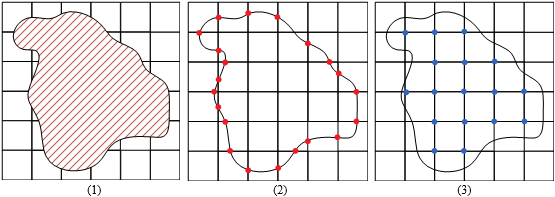
\includegraphics[width=10cm]  {3.png}} 
	\caption{Sampling process}
	\label{sample points}
\end{figure}
The procedure to construct the sample points set ${N_{sample}}$ is presented in Algorithm \ref{algorithm1}. Note that $n$ is number of program variables.


\begin{breakablealgorithm}\label{algorithm1}
	\caption{Construction of the sample points set $N_{sample}$ }
	\begin{algorithmic}[1] 
		\Require the $c_{assume}$, the $\varepsilon$ and the number $n$.          
		\Ensure return sample points set $N_{sample}$.
		\State Let $D=[\;]$ be an empty list;
		\State Let $N_{sample_{inside}}=[\;]$ be an empty list;
		\State Let $N_{sample_{bound}}=[\;]$ be an empty list;
		\State $d = \frac{\varepsilon }{{n\cdot{c_{assume}}}}$; \quad\quad//calculate the step $d$
		\Function{hypercube}{$n$,$d$}  
		\If{n==1}
		\State $i=d$;
		\While{$i\leq1-d$}
		\State append $[i]$ to $D$;
		\State $i += d$;
		\EndWhile
		\Else\;{$n>1$}
		\For{each $j$ in $hypercube(n-1,d)$}
		\State $i=d$;
		\While{$i\leq1-d$}
		\State append $[i]$ to $j$;
		\State append $[j]$ to $D$;
		\State$i+=d$;
		\EndWhile
		\EndFor
		\EndIf
		\State\Return $D$;
		\EndFunction
		\State$hypercube(n)$;
		\For{each $u$ in $D$}     \quad\quad //get the $N_{sample\_inside}$
		\If{$u$ in $U(\Omega)$}
		\State append $u$ to $N_{sample\_inside}$
		\EndIf
		\EndFor
		\For{each $u$ in $D$} \quad\quad //get the $N_{sample\_bound}$
		\For{$i:=1$ to $n$}
		\State Delete $u_{i}$ in $u$; 
		\State let $k=ln(\cfrac{u_{i}}{1-u_{i}})$ is the value to be solves;
		\For{$j:=1$ to $m$} \quad\quad // solve the intersections between the boundary of $U(\Omega)$ with hypercube
		\State$res=Solve(g_{j}((ln(\cfrac{u_{1}}{1-u_{1}})),(ln(\cfrac{u_{2}}{1-u_{2}})),\cdots,k,\cdots,(ln(\cfrac{u_{n}}{1-u_{n}})))\leq0)$
		\For{each $k$ in $res$} \quad\quad //tell the res whether is in $U(\Omega)$
		\If{$\stackrel{m}{{\bigwedge}\atop{{k=1}\atop{k\neq i}}}g_{k}(g_{j}((ln(\cfrac{u_{1}}{1-u_{1}})),(ln(\cfrac{u_{2}}{1-u_{2}})),\cdots,k,\cdots,(ln(\cfrac{u_{n}}{1-u_{n}})))\leq0)$}
		\State append $(u_{1},u_{2},\cdots,k,\cdots,u_{n})$ to $N_{sample\_bound}$;
		\EndIf
		\EndFor
		\EndFor
		\EndFor
		\EndFor
		\State append $N_{sample\_inside}$ $N_{sample\_bound}$ to $N_{sample}$
		\State \Return $N_{sample}$
	\end{algorithmic}
\end{breakablealgorithm}
\begin{rem}
	Given the value of $d$, one can construct $N_{sample}$ by Algorithm \ref{algorithm1}.
\end{rem}

The Theorem \ref{thm4} next will show that the union of neighborhoods of each points in $N_{sample}$ can cover $U(\Omega)$, if $U({\Omega})$ is a single connected region and ${N_{sample}}$ obtained by Algorithm \ref{algorithm1} is not empty.

Since the value of $d$ depends on $c_{assume}$ and $c_{assume}$ is given in advance, so when $U(\Omega)$ or one of connected branches of $U(\Omega)$ is the set in Figure \ref{the particular region}. Algorithm \ref{algorithm1} may not find $N_{sample}$ from the $s$.
\begin{figure}[H] 
	\center{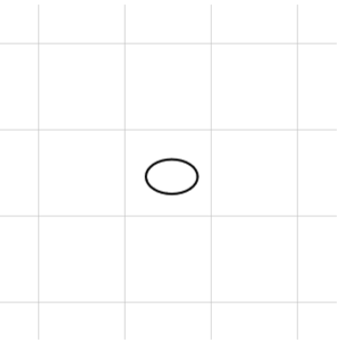
\includegraphics[width=5cm]  {4.png}} 
	\caption{\label{the particular region} The particular set $s$}
\end{figure}
When $U(\Omega )$ a simply connected region, and the sample point set ${N_{sample}}$ is not an empty set, we exclude this special case. So the ${N_{sample}}$ can cover the $U(\Omega )$. 

\begin{mythm}\label{thm4}
	Suppose $U(\Omega )$ is a simply connected region and ${N_{sample}} \ne \emptyset $. Let $U(\Omega )$ be the image set under $U(x)$ of $\Omega$. Then, for any a point $p$ in $U(\Omega)$, there exists $q$ in ${N_{sample}}$, such that $|p - q| \le \sqrt n d$.
\end{mythm}
\emph{Proof.}
For convenience, we next just consider the case when $n=2$, and the similar analysis is applicable for the general case. For $n = 2$, W.L.O.G, $U(\Omega )$ is an irregular region shown in (1) of Figure \ref{proof}. The $N_{sample}$ is shown in (2) of Figure \ref{proof}, where the red dots denote the points in ${N_{sample\_bound}}$ and the blue dots denote the points in ${N_{sample\_inside}}$.
\begin{figure}[htb] 
	\center{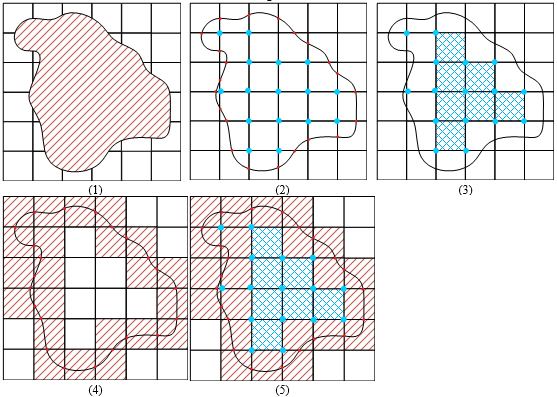
\includegraphics[width=15cm]  {5.png}} 
	\caption{\label{proof}Coverage processes}
\end{figure}
Then, from (5) in Figure \ref{proof}, we can see that the $U(\Omega )$ can be covered by a finite number of small squares with the length $d$. Let $H$ be the collection of finitely many squares. Clearly, we have $U(\Omega ) \subseteq H$.  The $H$ can be divided into two parts: $H_{boundary}$ and $H_{inside}$, where, $H_{boundary}$ denotes the set of squares which intersect with the boundary of $U(\Omega)$, and $H_{inside}$ denotes the set of squares which are completely contained in $U(\Omega)$. $H_{boundary}$ and $H_{inside}$ are shown in (3) and (4) of Figure \ref{proof}, respectively. And each square at least has one sample point in $N_{sample}$, thus, the union of neighborhoods of all points in ${N_{sample}}$ can cover these squares $H$. Since the $H$ covers the $U(\Omega )$, the union of neighborhoods of all points in ${N_{sample}}$ can cover $U(\Omega )$.$\square$

\begin{rem}
	Theorem \ref{thm4} proves that the union $\mathop  \cup \limits_{q \in {N_{sample}}} {\rm O}(q,\sqrt n d)$ of neighborhoods of each point in $N_{sample}$ can cover $U(\Omega)$, if $U({\Omega})$ is a single connected region.
\end{rem}

To sum up, by Theorem \ref{thm4} and Algorithm \ref{algorithm1}, we can find the points set $N_{sample}$ such that the union of the neighborhoods of each point in $N_{sample}$ can cover $U(\Omega )$. 
In what follows, we propose a method to build the train-set of neural network according to the \textbf{\emph{decreasing}} condition of ranking functions. 
\subsection{Train-set}
\label{Train-set}
To build the train-set, we need to build the inputs and outputs of neural network.
\subsubsection{The inputs of neural work}
\label{The inputs of neural work}
According to the \textbf{\emph{decreasing}} condition $r(u)-r(u')\ge c^+$ of ranking function, thus we need not only the value of $r(u)$, but also the value of $r(u')$, such that $r(u)-r(u')\ge c^+$. At the above steps, we have already got the sample points set ${N_{sample}}$ for $u$ by Algorithm \ref{algorithm1}. Thus, since $u$ is taken from $N_{sample}$ and $u' = U \circ f({U^{ - 1}}(u))$, we can get another sample points set $N'_{sample}$ about $u'$.

Let
\begin{equation}\label{equ:N_sample and N_sample'}
{\overline N_{sample}}  = {N_{sample}} \cup {{N'}_{sample}}
\end{equation}
is the sample points set for DNN.
Note that ${N_{sample}} = (u,1)$ and ${{N'}_{sample}} = (u',1)$, where $1$ is the bias term.
\subsubsection{The outputs of neural network}
\label{The outputs of neural network}
At the above steps, we get the ${\overline N _{sample}}$, which is the inputs of neural network. Next we need to determine an outputs for each sample point in ${\overline N _{sample}}$ according to the \textbf{\emph{decreasing}} condition.

According to the \textbf{\emph{decreasing}} condition of ranking functions, we construct train-set ${D_{train}} = \left\{ {(u,1,r(u))} \right\} \cup \left\{ {(u',1,r(u'))} \right\}$, such that $r(u) - r(u') > 0$.
For convenience, label output $\lambda$ for $u$ and another output $\lambda'$ for $u'$. To guarantee that $r(u) - r(u') > 0$, we set $\lambda  \in ({n_1},1)$ and $\lambda ' = \lambda  - l$, where $l \in ({n_2},{n_1})$ and $1 \ge {n_1} > {n_2}\ge 0$. Here $n_1$, $n_2$ are experimental tunable parameters. 

To summarize, the train-set $D_{train}$ consists of inputs and outputs, as follows:
\begin{table}[H]{\label{Dtrain}}
	\begin{center}
		\setlength{\abovecaptionskip}{0pt}   
		\setlength{\belowcaptionskip}{0pt}
		\caption{train-set $D_{train}$}
		\begin{tabular}{|l|l|l|}
			\hline
			\cline{1-1} \cline{3-3}
			inputs & \multirow{3}{*}{by DNN} & outputs   \\ \cline{1-1} \cline{3-3} 
			$(u,1)$  &                                     & $\lambda$  \\ \cline{1-1} \cline{3-3} 
			$(u',1)$ &                                     & $\lambda'$ \\ \cline{1-1} \cline{3-3} \hline
		\end{tabular}
	\end{center}
\end{table}
Note that $1$ is the bias term and the datas $(u,1,\lambda)$, $(u',1,\lambda')$ satisfy: $r(u)-r(u')=\lambda-\lambda'>0$.

The procedure to construct train-set ${D_{train}} = \{ (z,1,r(z)),z \in \overline N_{sample}\} $ is embedded in Algorithm 2. By this means, a candidate ranking function can be trained by DNN.
\begin{algorithm}[H] 
	\label{algorithm2}
	\caption{Construction of a train-set $D_{train}$}
	\begin{algorithmic}[1] %??????
		\Require the sample points set $N_{sample}$, the guard condition,the update function $x_{i}'=f_{i}(x)$, the positive number $n_{1}$ and $n_{2}$.          
		\Ensure return $D_{train}$
		\State $D_{train}=[\;]$;
		\For{each $u$ in $N_{sample}$}
		\State append $1$ to u; // add the bias term
		\State $\lambda=random(n_{1},1)$; // label the output $\lambda$ for $u$
		\State append $[\lambda]$ to $u$;
		\State append $u$ to $D_{train}$;
		\State $u_{i}'=\cfrac{1}{1+e^{f_{i}(ln(\cfrac{u_{1}}{1-u_{1}}),ln(\cfrac{u_{2}}{1-u_{2}}),\cdots,ln(\cfrac{u_{n}}{1-u_{n}}))}}$; // calculate $u'$
		\State append $1$ to $u'$;
		\State $l = random({n_2},{n_1})$;
		\State $\lambda'=\lambda-l$; //label output $\lambda'$ for $u'$
		\State append $[\lambda']$ to $u'$;
		\State append $u'$ to $D_{train}$;
		\EndFor
		\State \Return{$D_{train}$}
	\end{algorithmic}
\end{algorithm}
Note that ${n_1} \in [0,1]$ and ${n_2} \in [0,{n_1}]$. In most of our experiments, we take ${n_1} = 0.5$ and ${n_{\rm{2}}} = 0$. However, in some cases, we may adjust the ${n_1}$ and ${n_2}$ to achieve the best training effect.

\begin{exam}\label{exm3}
	Let $\Omega$ be a set defined in Example 1 and let $U(x)=(m(x_1),m(x_2))$ be a mapping defined in Example 2. That is,
	
	$$\begin{array}{l}
	{u_1} = \frac{1}{{1 + {e^{ - {x_1}}}}},{u_2} = \frac{1}{{1 + {e^{ - {x_2}}}}}\\
	{{u_1}'} = \frac{1}{{1 + {e^{ - {{x_1}'}}}}} = \frac{1}{{1 + {e^{ - ({x_1} - {x_2}^2 + 1)}}}},{{u_2}'} = \frac{1}{{1 + {e^{ - {{x_2}'}}}}} = \frac{1}{{1 + {e^{ - ({x_2} + {x_1}^2 - 1)}}}}
	\end{array}$$
	
	So we have the image set $U(\Omega)$ under $U(x)$ of $\Omega$:
	$$U(\Omega ) = \{ ({u_1},{u_2}) \in {R^2}:{(\ln (\frac{{{u_1}}}{{1 - {u_1}}}))^2} + {(\ln (\frac{{{u_2}}}{{1 - {u_2}}}))^2} \le 1\} $$
	
	Since this loop only has two variables, the $n=2$. And we set ${c_{assume}} = 2.5$ and $\lambda  = 0.01$.
	
	Then, the $d = \frac{\lambda }{{n\cdot{c_{assume}}}} = 0.002$.
	
	Besides, we set $n_1=0.5$ and $n_2=0.2$. The train-set $D_{train}$ is as follows:
	
	
	\begin{table}[H]{\label{output of Dtrain}}\label{tabel2}
		\begin{center}
			\setlength{\abovecaptionskip}{0pt}   
			\setlength{\belowcaptionskip}{0pt}
			\caption{the output of $D_{train}$}
			
			\begin{tabular}{|c|lllllll|}
				\hline
				\multirow{3}{*}{$({u_{\rm{1}}},{u_2},1)$} & 0.27333333 & 0.27333333 & 0.28       & $\cdots $ & 0.73       & 0.73       & 0.73       \\
				& 0.44777785 & 0.55222215 & 0.418576   & $\cdots $ & 0.52       & 0.522      & 0.524      \\
				& 1          & 1          & 1          & $\cdots $ & 1          & 1          & 1          \\ \hline
				\multirow{3}{*}{$({u'_1},{u'_2},1)$} & 0.49456765 & 0.49456765 & 0.48688954 & $\cdots $ & 0.87955424 & 0.87941145 & 0.87925482 \\
				& 0.43693574 & 0.54133016 & 0.39254807 & $\cdots $ & 0.51732226 & 0.5193231  & 0.52132403 \\
				& 1          & 1          & 1          & $\cdots $ & 1          & 1          & 1          \\ \hline
				$\lambda $& 0.9359949  & 0.54966248 & 0.9203678  & $\cdots $ & 0.7432145  & 0.91482292 & 0.86196221 \\ \hline
				$\lambda '$& 0.61006867 & 0.21434009 & 0.49003298 & $\cdots $ & 0.35222001 & 0.54831943 & 0.43670077 \\ \hline
			\end{tabular}
		\end{center}
	\end{table}
	
\end{exam} 

\subsection{test-set}
\label{test-set}
From Theorem \ref{thm4}, we know that the $N_{sample}$ obtained by Algorithm \ref{algorithm1} can cover $U(\Omega)$, when $U(\Omega)$ is a simply connected region. Thus, in order to verify if each point $(u,u') \in {N_{sample}} \times {{N'}_{sample}}$ satisfies $r(u)-r(u')\ge c^+$, then the test-set is  ${N_{sample}} \times {{N'}_{sample}}$.

In the experiments, we take the points $(u,u')$ from ${N_{sample}} \times {{N'}_{sample}}$ one by one and verify them if $r(u) - r(u') \ge \varepsilon > 0$. If $r(u) - r(u') \ge \varepsilon $ holds for all points in ${N_{sample}} \times {{N'}_{sample}}$, then all points in $N_{sample}$ satisfy the decreasing condition. We will output the weights to get a candidate ranking function. Here, the value of $\varepsilon $ should be given in advance, which can be adjusted. And the smaller $\varepsilon $ is, the greater the probability of all points satisfy $r(u) - r(u') \ge \varepsilon $.

Algorithm 3 describes the process of using neural network to detect the candidate ranking function $r(u)$.
\begin{algorithm}[H]
	\label{algorithm3}
	\caption{Synthesis of candidate ranking functions}
	\begin{algorithmic}[1] %??????
		\Require a train-set ${D}$,the network structure, the sigmoid activation function.          
		\Ensure return the weights $w_i$ and $w_{ji}$.
		\State Choose the tunable parameters $\varepsilon $ and $c_{assume}$.
		\State Construct $N_{sample}$ by Algorithm 1;
		\State Construct $D_{train}$ by Algorithm 2;
		\State Training by DNN through the train-set $D_{train}$;
		\If{the accuracy of test set == $1$}
		\State \Return the weights $w_i$ and $w_{ji}$;
		\Else
		\State adjust the tunable parameters and  optimization algorithm;
		\EndIf 
	\end{algorithmic}
\end{algorithm}

\section{Exact Verification}
\label{Exact Verification}
By Algorithm 3, we can get the value of $w_i$ and $w_{ji}$, which reduce a candidate ranking function $r(u)$ over $U(\Omega)$. In this section, we will check if the $r(u)$ is a ranking function. To verify $r(u)$, we propose a new method instead of symbolic computation like $Z3$ and $SMT-solver$. At first, in Section \ref{Verification Process}, we put forward a proposition, which states that while $c < c_{assume}$ and all the points in ${N_{sample}}$ obtained by Algorithm 1 satisfy $p(u)=r(u) - r(U \circ f \circ {U^{ - 1}}(u)) \ge \varepsilon  > 0$, the function $r(u)$ satisfies the \textbf{\emph{decreasing}} condition of ranking functions over $U(\Omega )$. And in Section \ref{Computation}, we will propose a method to calculate the upper bound $c$ of ${\rm{|}}\bigtriangledown(r(u) - r(u')|$ in Proposition 1.
\subsection{Verification Process} 
\label{Verification Process}
The verification method includes two steps. First, we need to prove the union of all neighborhood with radius $\sqrt n d$ of each point in $N_{sample}$ can cover the $U(\Omega )$, which has been implemented by Theorem \ref{thm4} and its Remark. Then, we need to prove the points in the neighborhood of each point in $N_{sample}$ satisfy the \textbf{\emph{decreasing}} condition of ranking functions, i.e., for any point $\alpha$ in $N_{sample}$, $r(u) - r(U \circ f \circ {U^{ - 1}}(u)) \ge c^+ $ holds for any $u \in {\rm O}(\alpha,\sqrt n d)$, this guarantees that $r(u) - r(U \circ f \circ {U^{ - 1}}(u)) \ge c^+ $ holds for any $u$ in $U(\Omega)$, since the union of neighborhoods of all points in $N_{sample}$ can cover $U(\Omega)$.

By Theorem \ref{thm3}, we know that if ${\rm{|}}\bigtriangledown(r(u) - r(U \circ f({U^{ - 1}}(u))))|$ have a upper bound $c$ and $\alpha$ is a point $\alpha $ in $N_{sample}$ satisfies $r(\alpha) - r(U \circ f({U^{ - 1}}(\alpha)))\ge \varepsilon$, then any point $\theta $ in the neighborhood ${\rm O}(\alpha,\sqrt n d)$ satisfies $r(\theta) - r(U \circ f({U^{ - 1}}(\theta)))\ge\varepsilon-ndc$. Next, according to the \textbf{\emph{decreasing}} condition, we need to give a condition to ensure that $\varepsilon-ndc$ is a positive number. 

The Proposition 1 will show that when step $d = \frac{\varepsilon }{{n\cdot{c_{assume}}}}$ and each point in ${N_{sample}}$ satisfies the \textbf{\emph{decreasing}} condition, then each point in $U(\Omega)$ will satisfy the \textbf{\emph{decreasing}} condition too, if $c < {c_{assume}}$.



\newtheorem{myprop}{Proposition}
\begin{myprop} \label{prop}
	If $c < {c_{assume}}$ and each point $\alpha $ in ${N_{sample}}$ satisfy the \textbf{\emph{decreasing}} condition $r(\alpha)-r(U \circ f({U^{ - 1}}(\alpha))) \ge \varepsilon  > 0$, then $\forall u  \in U(\Omega)$, we have $r(u)-r(U \circ f({U^{ - 1}}(u))) \ge \varepsilon  - ndc > 0$.
\end{myprop}
\emph{Proof.}

By Theorem \ref{thm3}, we have already proved that if each point $\alpha $ in ${N_{sample}}$ satisfies $r(\alpha)-r(U \circ f({U^{ - 1}}(\alpha))) \ge \varepsilon  > 0$, then $\forall \theta  \in {\rm O}(\alpha,\sqrt n d)$, we have $r(\theta)-r(U \circ f({U^{ - 1}}(\theta))) \ge \varepsilon  - ndc$.

By (\ref{equ:d}), since $$d = \frac{\varepsilon }{{n\cdot{c_{assume}}}}$$
substitute $d$ into $p(\theta ) \ge \varepsilon  - ndc$, we have $\forall \theta  \in {\rm O}(\alpha,\sqrt n d)$
\begin{equation}\label{equ:LMT(positive)}
r(\theta)-r(U \circ f({U^{ - 1}}(\theta))) \ge \varepsilon  - ndc = \varepsilon  - n\frac{\varepsilon }{{n\cdot{c_{assume}}}}c = \varepsilon  - \varepsilon \frac{c}{{{c_{assume}}}} = \varepsilon (\frac{{{c_{assume}} - c}}{{{c_{assume}}}}).
\end{equation}
Owing to $c < {c_{assume}}$, we have $r(\theta)-r(U \circ f({U^{ - 1}}(\theta))) \ge \varepsilon (\frac{{{c_{assume}} - c}}{{{c_{assume}}}}) > {\rm{0}}$.  

by above, we know that for any point $\alpha$ in $N_{sample}$, $r(u) - r(U \circ f \circ {U^{ - 1}}(u)) \ge \varepsilon -ndc > 0$ holds for any $u \in {\rm O}(\alpha,\sqrt n d)$. By Theorem \ref{thm4} and its Remark, we know that the union of neighborhoods of all points in $N_{sample}$ can cover $U(\Omega)$. Thus, $r(u) - r(U \circ f \circ {U^{ - 1}}(u)) \ge \varepsilon - ndc > 0 $ holds for any $u$ in $U(\Omega)$. $\square$


\begin{rem}
	By Theorem \ref{thm3} and Proposition 1, we can prove that when $d = \frac{\varepsilon }{{n\cdot{c_{assume}}}}$, if $c < {c_{assume}}$, the function $r(u)$ satisfies the \textbf{\emph{decreasing}} condition of ranking functions, i.e., $\forall u  \in U(\Omega)$, we have $r(u)-r(U \circ f({U^{ - 1}}(u))) \ge \varepsilon  - ndc > 0$. Owing to $r(u)$ satisfies the bounded function naturally by Theorem \ref{thm2}, thus $r(u)$ is exactly a ranking function over $U(\Omega )$. By Theorem \ref{thm1}, since $r=R\circ U^{-1}$ and $u=U(x)$, $r(u)=R\circ U^{-1} U(x) = R(x)$, which is a ranking function over $\Omega$. By our verification method, different from existing methods, the verification of candidate ranking function is no longer limited by the verification tools such as $Z3$.
\end{rem}

To check if the candidate ranking function $r(u)$ is a real ranking function, by Proposition 1 and its Remark, we need to compute the value of $c$ and check if $c<c_{assume}$. In the following, we will illustrate how to compute the value of $c$.
\subsection{Computation of $c$}
\label{Computation}
In this section, we will  propose a method to get the upper bound $c$ of $\left| \bigtriangledown{(r(u) - r(u'))} \right|$, where $r(u)$ is a candidate ranking function of following form.

$$r(u) = \frac{1}{{1 + {e^{ - (\sum\limits_{i = 1}^l {{w_i}\frac{1}{{1 + {e^{ - (\sum\limits_{j = 1}^{n+1} {{w_{ji}}\cdot{u_j}} )}}}}} )}}}}$$
where the value of $w_i$ and $w_{ji}$ have been obtained by Algorithm 3.
Since  $u' = U \circ f({U^{ - 1}}(u))$, 

\begin{equation}\label{equ:|r(u)-r(u')|}
\left|\bigtriangledown {(r(u) - r(u'))} \right|{\rm{ = }}\left| {\bigtriangledown r(u) - \bigtriangledown r \circ U \circ f \circ {U^{ - 1}}(u)} \right|{\rm{ = }}\left| {\left( \begin{array}{c}
	\frac{{\partial r(u)}}{{\partial {u_1}}}\\
	\frac{{\partial r(u)}}{{\partial {u_2}}}\\
	\vdots \\
	\frac{{\partial r(u)}}{{\partial {u_n}}}
	\end{array} \right) - \left( \begin{array}{c}
	\frac{{\partial r \circ U \circ f \circ {U^{ - 1}}(u)}}{{\partial {u_1}}}\\
	\frac{{\partial r \circ U \circ f \circ {U^{ - 1}}(u)}}{{\partial {u_2}}}\\
	\vdots \\
	\frac{{\partial r \circ U \circ f \circ {U^{ - 1}}(u)}}{{\partial {u_n}}}
	\end{array} \right)} \right|.
\end{equation}

Owing to $[sigmoid(z)]' = sigmoid(z)\cdot(1 - sigmoid(z))$ and  $sigmoid(z) \in (0,1)$, thus, $[sigmoid(z)]' \in (0,\frac{1}{4})$.
Thus, we have
\begin{equation}\label{equ:sigmoid(z)}
[sigmoid(z)]' = \frac{{{e^{ - z}}}}{{{{(1 + {e^{ - z}})}^2}}} \in (0,\frac{1}{4}).
\end{equation}
By (\ref{equ:sigmoid(z)}), we have
\begin{equation}\label{equ:|r(u)/u_k|}
\begin{array}{l}
\left| {\frac{{\partial r(u)}}{{\partial {u_k}}}} \right| = \left| {(\frac{1}{{1 + {e^{ - (\sum\limits_{i = 1}^l {{w_i}\frac{1}{{1 + {e^{ - (\sum\limits_{j = 1}^{n+1} {{w_{ji}}\cdot{u_j}} )}}}}} )}}}})'\cdot\frac{{\partial \sum\limits_{i = 1}^l {{w_i}\frac{1}{{1 + {e^{ - (\sum\limits_{j = 1}^{n+1} {{w_{ji}}\cdot{u_j}} )}}}}} }}{{\partial {u_k}}}} \right|\\
\quad \;\;\;\quad \; = \left| {(\frac{1}{{1 + {e^{ - (\sum\limits_{i = 1}^l {{w_i}\frac{1}{{1 + {e^{ - (\sum\limits_{j = 1}^{n+1} {{w_{ji}}\cdot{u_j}} )}}}}} )}}}})'} \right|\cdot\left| {\sum\limits_{i = 1}^l {[{w_i}(\frac{1}{{1 + {e^{ - (\sum\limits_{j = 1}^{n+1} {{w_{ji}}\cdot{u_j}} )}}}}} )'\cdot{w_{ki}}]} \right|\\
\quad \;\;\;\quad \; \le \frac{1}{{16}}\sum\limits_{i = 1}^l {\left| {{w_i}\cdot{w_{ki}}} \right|} ,k \in (1,2, \cdots ,n)
\end{array}
\end{equation}
\begin{equation}\label{equ:|r(u')/u_k|}
\begin{array}{l}
\left| {\frac{{\partial r \circ U \circ f \circ {U^{ - 1}}(u)}}{{\partial {u_k}}}} \right| = \left| {(\frac{1}{{1 + {e^{ - (\sum\limits_{i = 1}^l {{w_i}\frac{1}{{1 + {e^{ - ({w_{(n + 1)i}} + \sum\limits_{j = 1}^n {{w_{ji}}\cdot(m \circ {f_j} \circ {U^{ - 1}}(u))} )}}}}} )}}}})'\cdot\frac{{\partial \sum\limits_{i = 1}^l {{w_i}\frac{1}{{1 + {e^{ - ({w_{(n + 1)i}} + \sum\limits_{j = 1}^n {{w_{ji}}\cdot(m \circ {f_j} \circ {U^{ - 1}}(u))} )}}}}} }}{{\partial {u_k}}}} \right|\;\\
\;\;\quad \quad \,\quad \quad \quad \quad \;= \left| {(\frac{1}{{1 + {e^{ - (\sum\limits_{i = 1}^l {{w_i}\frac{1}{{1 + {e^{ - ({w_{(n + 1)i}} + \sum\limits_{j = 1}^n {{w_{ji}}\cdot(m \circ {f_j} \circ {U^{ - 1}}(u))} )}}}}} )}}}})'} \right|\\\;\;\quad \quad \;\;\quad \quad \;\;\quad \quad \;\cdot\left| {\sum\limits_{i = 1}^l {{w_i}[(\frac{1}{{1 + {e^{ - ({w_{(n + 1)i}} + \sum\limits_{j = 1}^n {{w_{ji}}\cdot(m \circ {f_j} \circ {U^{ - 1}}(u))} )}}}}} )'\cdot\frac{{\partial \sum\limits_{j = 1}^n {{w_{ji}}\cdot(m \circ {f_j} \circ {U^{ - 1}}(u))} }}{{\partial {u_k}}}]} \right|\\
\;\;\quad \quad \,\quad \quad \quad \quad \; \le \frac{1}{{16}}\sum\limits_{i = 1}^l {\left| {{w_i}\cdot\sum\limits_{j = 1}^n {{w_{ji}}\cdot\left| {\frac{{\partial (m \circ {f_j} \circ {U^{ - 1}}(u))}}{{\partial {u_k}}}} \right|} } \right|} ,k \in (1,2, \cdots ,n).
\end{array}
\end{equation}

For $\left| {\frac{{\partial r(u)}}{{\partial {u_k}}}} \right|$ in (\ref{equ:|r(u)/u_k|}), since $w_i$ and $w_{ji}$ are known, the upper bound of $\left| {\frac{{\partial r(u)}}{{\partial {u_k}}}} \right|$ is known. For $\left| {\frac{{\partial r \circ U \circ f \circ {U^{ - 1}}(u)}}{{\partial {u_k}}}} \right|$ in (\ref{equ:|r(u')/u_k|}), if the upper bound of ${\left| {\frac{{\partial (m \circ {f_j} \circ {U^{ - 1}}(u))}}{{\partial {u_k}}}} \right|}$ can be obtained, then the upper bound of $\left| {\frac{{\partial r \circ U \circ f \circ {U^{ - 1}}(u)}}{{\partial {u_k}}}} \right|$ is derived.

Next, based on the the upper bound of $\frac{{\partial r(u)}}{{\partial {u_i}}}$ and $\frac{{\partial r \circ U \circ f \circ {U^{ - 1}}(u)}}{{\partial {u_i}}}$, we propose a method to calculate the upper bound $c$ of $\left| \bigtriangledown{(r(u) - r(u'))} \right|$.

\textbf{\emph{Method.}}
\begin{equation}\label{equ:method(u)}
\begin{array}{l}
\left| {\bigtriangledown(r(u) - r \circ U \circ f \circ {U^{ - 1}}(u))} \right| = \left| {\left( \begin{array}{c}
	\frac{{\partial r(u)}}{{\partial {u_1}}}\\
	\frac{{\partial r(u)}}{{\partial {u_2}}}\\
	\vdots \\
	\frac{{\partial r(u)}}{{\partial {u_n}}}
	\end{array} \right) - \left( \begin{array}{c}
	\frac{{\partial r \circ U \circ f \circ {U^{ - 1}}(u)}}{{\partial {u_1}}}\\
	\frac{{\partial r \circ U \circ f \circ {U^{ - 1}}(u)}}{{\partial {u_2}}}\\
	\vdots \\
	\frac{{\partial r \circ U \circ f \circ {U^{ - 1}}(u)}}{{\partial {u_n}}}
	\end{array} \right)} \right|\;\\
\quad \quad \quad \quad \quad \quad \quad \quad \quad \,\quad \quad \quad\quad\,\; \le \sum\limits_{{\rm{i}} \in {\rm{(1,2,}} \cdots {\rm{,n)}}} {\left| {\frac{{\partial r(u)}}{{\partial {u_i}}}} \right|}  + \sum\limits_{{\rm{i}} \in {\rm{(1,2,}} \cdots {\rm{,n)}}} {\left| {\frac{{\partial r \circ U \circ f \circ {U^{ - 1}}(u)}}{{\partial {u_i}}}} \right|}. 
\end{array}
\end{equation}

By (\ref{equ:|r(u)/u_k|}) and (\ref{equ:|r(u')/u_k|}), we can get the upper bound of $\left| {\frac{{\partial r(u)}}{{\partial {u_k}}}} \right|$ and $\left| {\frac{{\partial r \circ U \circ f \circ {U^{ - 1}}(u)}}{{\partial {u_k}}}} \right|$. Then by (\ref{equ:method(u)}), we get the upper bound $c$ of $\left| \bigtriangledown{(r(u) - r(u'))} \right|$.

It can be seen from (\ref{equ:method(u)}) that the upper bound $c$ of $\left| \bigtriangledown(r(u) - r \circ U \circ f \circ {U^{ - 1}}(u)) \right|$ depends on the upper bound of $\left| {\frac{{\partial r \circ U \circ f \circ {U^{ - 1}}(u)}}{{\partial {u_k}}}} \right|$. By (\ref{equ:|r(u')/u_k|}), we know that the upper bound of $\left| {\frac{{\partial r \circ U \circ f \circ {U^{ - 1}}(u)}}{{\partial {u_k}}}} \right|$ depends on the upper bound of ${\left| {\frac{{\partial (m \circ {f_j} \circ {U^{ - 1}}(u))}}{{\partial {u_k}}}} \right|}$. Thus, the upper bound $c$ depends on the upper bound of ${\left| {\frac{{\partial (m \circ {f_j} \circ {U^{ - 1}}(u))}}{{\partial {u_k}}}} \right|}$. Next, we will discuss when the upper bound of ${\left| {\frac{{\partial (m \circ {f_j} \circ {U^{ - 1}}(u))}}{{\partial {u_k}}}} \right|}$ is computable.

Since $x=U^{-1}(u)$, $x_{j}'=f_{j}(x)$ and ${x_i} = m^{-1}(x_i)=\ln (\frac{{{u_i}}}{{1 - {u_i}}})$, we have 
\begin{equation}{\label{equ:computing c}}
\begin{array}{l}
\left| {\frac{{\partial (m \circ {f_j} \circ {U^{ - 1}}(u))}}{{\partial {u_k}}}} \right| = \left| {(m \circ {f_j} \circ {U^{ - 1}}(u))'\cdot\frac{{\partial ({f_j} \circ {U^{ - 1}}(u))}}{{\partial {u_k}}}} \right|\\
\quad \quad \;\;\quad \quad \;\;\quad \quad \, = \left| {(m \circ {f_j}(x))'\cdot\frac{{\partial ({f_j}(x))}}{{\partial {x_k}}}\cdot\frac{{\partial {x_k}}}{{\partial {u_k}}}} \right|\\
\quad \quad \;\;\quad \quad \;\;\quad \quad\,  = \left| {(m \circ {f_j}(x))'\cdot\frac{{\partial ({f_j}(x))}}{{\partial {x_k}}}\cdot\frac{1}{{{u_k}(1 - {u_k})}}} \right|\\
\quad \quad \;\;\quad \quad \;\;\quad \quad\,  = \left| {\frac{{m({x_{j}'})(1 - m({x_{j}'}))}}{{m({x_k})(1 - m({x_k}))}}\cdot\frac{{\partial ({f_j}(x))}}{{\partial {x_k}}}} \right|\\
\quad \quad \;\;\quad \quad \;\;\quad \quad  \,= \left| {\frac{{{e^{{x_k}}} + {e^{ - {x_k}}} + 2}}{{{e^{{x_{j}'}}} + {e^{ - {x_{j}'}}} + 2}}\cdot\frac{{\partial ({f_j}(x))}}{{\partial {x_k}}}} \right|.
\end{array}
\end{equation}

Next, we will illustrate how to compute the upper bound of ${\left| {\frac{{\partial (m \circ {f_j} \circ {U^{ - 1}}(u))}}{{\partial {u_k}}}} \right|}$. There are two cases to consider:

\textbf{\emph{A.}} The $\mathcal{H}$ is bounded and ${\frac{{\partial ({f_j}(x))}}{{\partial {x_k}}}}$ is continuous. Since ${\frac{{{e^{{x_k}}} + {e^{ - {x_k}}} + 2}}{{{e^{{x_{j}'}}} + {e^{ - {x_{j}'}}} + 2}}}$ and ${\frac{{\partial ({f_j}(x))}}{{\partial {x_k}}}}$ is continuous and $\mathcal{H}$ is bounded, then $\left| {\frac{{{e^{{x_k}}} + {e^{ - {x_k}}} + 2}}{{{e^{{x_{j}'}}} + {e^{ - {x_{j}'}}} + 2}}} \right|$ and $\left| {\frac{{\partial ({f_j}(x))}}{{\partial {x_k}}}} \right|$ have upper bounds over $\mathcal{H}$. Thus, we can compute the upper bound of ${\left| {\frac{{\partial (m \circ {f_j} \circ {U^{ - 1}}(u))}}{{\partial {u_k}}}} \right|}$ over $\mathcal{H}$.

\begin{exam}\label{exm4}
	Consider the loop in Example 1:
	$$\begin{array}{l}
	while\;\;{x_1}^2 + {x_2}^2 \le 1\quad do\\
	{{x_1}'} = {x_1} - {x_2}^2 + 1,{{x_2}'} = {x_2} + {x_1}^2 - 1
	\end{array}$$
	
	Let $\mathcal{H} =\left\{ {({x_1},{x_2}):1 \ge {x_1} \ge -1,\ge {x_2} \ge -1} \right\}$. And we can get $\frac{{\partial {{x_1}'}}}{{\partial {x_1}}} = 1$, $\frac{{\partial {{x_1}'}}}{{\partial {x_2}}} = -2x_2$, $\frac{{\partial {{x_2}'}}}{{\partial {x_1}}} = 2x_1$ and $\frac{{\partial {{x_2}'}}}{{\partial {x_2}}} = 1$. 
	
	Thus, by (\ref{equ:computing c}),
	
	$\left| {\frac{{\partial (m \circ {f_1} \circ {U^{ - 1}}(u))}}{{\partial {u_1}}}} \right| = \left| {\frac{{{e^{{x_1}}} + {e^{ - {x_1}}} + 2}}{{{e^{{x_1}^\prime }} + {e^{ - {x_1}^\prime }} + 2}}\cdot1} \right| \le \left| {\frac{{{e^1} + {e^{ - 1}} + 2}}{{{e^0} + {e^0} + 2}}} \right| \le 1.28,$
	
	$\left| {\frac{{\partial (m \circ {f_1} \circ {U^{ - 1}}(u))}}{{\partial {u_2}}}} \right| = \left| {\frac{{{e^{{x_2}}} + {e^{ - {x_2}}} + 2}}{{{e^{{x_1}^\prime }} + {e^{ - {x_1}^\prime }} + 2}} \cdot ( - 2{x_2})} \right| \le \left| {\frac{{{e^1} + {e^{ - 1}} + 2}}{{{e^0} + {e^0} + 2}} \cdot 2} \right| \le 2.55,$
	
	$\left| {\frac{{\partial (m \circ {f_2} \circ {U^{ - 1}}(u))}}{{\partial {u_1}}}} \right| = \left| {\frac{{{e^{{x_2}}} + {e^{ - {x_2}}} + 2}}{{{e^{{x_2}^\prime }} + {e^{ - {x_2}^\prime }} + 2}} \cdot 2{x_1}} \right| \le \left| {\frac{{{e^1} + {e^{ - 1}} + 2}}{{{e^0} + {e^0} + 2}} \cdot 2} \right| \le 2.55,$
	
	$\left| {\frac{{\partial (m \circ {f_2} \circ {U^{ - 1}}(u))}}{{\partial {u_2}}}} \right| = \left| {\frac{{{e^{{x_1}}} + {e^{ - {x_1}}} + 2}}{{{e^{{x_2}^\prime }} + {e^{ - {x_2}^\prime }} + 2}} \cdot 1} \right| \le \left| {\frac{{{e^1} + {e^{ - 1}} + 2}}{{{e^0} + {e^0} + 2}}} \right| \le 1.28.$
	
	Thus, by (\ref{equ:|r(u')/u_k|}), we can get the upper bound of $\left| {\frac{{\partial r \circ U \circ f \circ {U^{ - 1}}(u)}}{{\partial {u_k}}}} \right|$. Then, by (\ref{equ:method(u)}), we can get the upper bound of  $\left| \bigtriangledown{(r(u) - r(u'))} \right|$.
	
\end{exam}

\textbf{\emph{B.}} The $\mathcal{H}$ is not bounded and ${f_j}(x)$ is linear, by (\ref{equ:computing c}), we just need to discuss whether the ${\frac{{{e^{{x_k}}} + {e^{ - {x_k}}} + 2}}{{{e^{{x_{j}'}}} + {e^{ - {x_{j}'}}} + 2}}}$ has a upper bound over $\mathcal{H}$.

It is easy to see that the function $y = {e^x} + {e^{ - x}} + 2$ monotonically decreases when $x \le 0$ and monotonically increases when $x > 0$. Thus, when $x_{j}'>x_k>0$ or $x_{j}' < x_k < 0$, ${{e^{x_{j}'}} + {e^{ - {x_{j}'}}} + 2} > {{e^{{x_k}}} + {e^{ - {x_k}}} + 2}$. The upper bound of $\left| {\frac{{{e^{{x_k}}} + {e^{ - {x_k}}} + 2}}{{{e^{{x_{j}'}}} + {e^{ - {x_{j}'}}} + 2}}} \right|$ is 1. 

Next, we take an example to illustrate this, as follows:
\begin{exam}\label{exm5}
	Consider the following loop from \cite{ben2017multiphase}:
	$$\begin{array}{l}
	while\,{x_1} > 0,{x_1} \le {x_2}\;\;do\,\\
	{{x_1}'} = 2{x_1},{{x_2}'} = {x_2} + 1
	\end{array}$$
	
	Let $\mathcal{H} =\left\{ {({x_1},{x_2}):{x_1} > 0,{x_2} \ge 0} \right\}$. And we can get $\frac{{\partial {{x_1}'}}}{{\partial {x_1}}} = 2$, $\frac{{\partial {{x_1}'}}}{{\partial {x_2}}} = 0$, $\frac{{\partial {{x_2}'}}}{{\partial {x_1}}} = 0$ and $\frac{{\partial {{x_2}'}}}{{\partial {x_2}}} = 1$.
	
	Thus, by (\ref{equ:computing c}), 
	$\left| {\frac{{\partial (m \circ {f_1} \circ {U^{ - 1}}(u))}}{{\partial {u_1}}}} \right| = \left| {\frac{{{e^{{x_1}}} + {e^{ - {x_1}}} + 2}}{{{e^{{x_1}' }} + {e^{ - {x_1}' }} + 2}}\cdot 1} \right|.$
	
	Since $x_{1}'=2x_1>x_1$ when $x_1>0$, ${{e^{x_{1}'}} + {e^{ - {x_{1}'}}} + 2} > {{e^{{x_1}}} + {e^{ - {x_1}}} + 2}$. The upper bound of $\left| {\frac{{{e^{{x_1}}} + {e^{ - {x_1}}} + 2}}{{{e^{{x_{1}'}}} + {e^{ - {x_{1}'}}} + 2}}} \right|$ is 1. Thus, the upper bound of $\left| {\frac{{\partial (m \circ {f_1} \circ {U^{ - 1}}(u))}}{{\partial {u_1}}}} \right|$ is 2.
	
	$\left| {\frac{{\partial (m \circ {f_1} \circ {U^{ - 1}}(u))}}{{\partial {u_2}}}} \right| = \left| {\frac{{{e^{{x_2}}} + {e^{ - {x_2}}} + 2}}{{{e^{{x_1}' }} + {e^{ - {x_1}' }} + 2}}\cdot 0} =0\right|$
	and
	$\left| {\frac{{\partial (m \circ {f_2} \circ {U^{ - 1}}(u))}}{{\partial {u_1}}}} \right| = \left| {\frac{{{e^{{x_1}}} + {e^{ - {x_1}}} + 2}}{{{e^{{x_2}' }} + {e^{ - {x_2}' }} + 2}}\cdot 0} =0\right|.$
	
	$\left| {\frac{{\partial (m \circ {f_2} \circ {U^{ - 1}}(u))}}{{\partial {u_2}}}} \right| = \left| {\frac{{{e^{{x_1}}} + {e^{ - {x_1}}} + 2}}{{{e^{{x_2}' }} + {e^{ - {x_2}' }} + 2}}\cdot 1} \right|.$
	
	Since $x_{2}'=x_2+1>x_2$, ${{e^{x_{2}'}} + {e^{ - {x_{2}'}}} + 2} > {{e^{{x_2}}} + {e^{ - {x_2}}} + 2}$. The upper bound of $\left| {\frac{{{e^{{x_2}}} + {e^{ - {x_2}}} + 2}}{{{e^{{x_{2}'}}} + {e^{ - {x_{2}'}}} + 2}}} \right|$ is 1. Thus, the upper bound of $\left| {\frac{{\partial (m \circ {f_2} \circ {U^{ - 1}}(u))}}{{\partial {u_2}}}} \right|$ is 1.
	
\end{exam}

By using the method, we can get an upper bound $c$ of $\left| \bigtriangledown{(r(u) - r(u'))} \right|$ in some case. Then we compare $c$ with ${c_{assume}}$ to determine whether $r(u)$ is the ranking function over $U(\Omega )$.

To sum up, we can elicit the process of the algorithm, which embedded in Algorithm 4. 
\begin{algorithm}[H]\label{algorithm4}
	\caption{Synthesis of ranking functions}
	\begin{algorithmic}[1] %??????
		\Require a train-set ${D_{train}}$,the network structure.            
		\Ensure return the ranking function $R(x)$.
		\State Choose the tunable parameters $\varepsilon$ and $c_{assume}$;
		\State Calculate the step size $d$: $d=\cfrac{\varepsilon}{n\cdot c_{assume}}$;
		\State Construct $N_{sample}$ by Algorithm 1;
		\State Construct a train-set $D_{train}$ by Algorithm 2;
		\State Detect the candidate ranking function $r(u)$ by Algorithm 3;
		\State Compute the upper bound $c$;
		\If{$c<c_{assume}$}
		\State \Return $R(x)$;
		\Else
		\State adjust $c_{assume}$ and the tunable parameters to train again;
		\EndIf
	\end{algorithmic}
\end{algorithm}
\begin{rem}
	In our experiments, in general, if $c$ obtained by the method states in Section \ref{Computation} still does not satisfy $c < c_{assume}$, then we increase the value of $c_{assume}$. The process may not be terminating. Thus, in our experiment, to guarantee the process is terminating, we limit the number of sample points does not exceed $10^7$. At the same time, when $c_{assume}$ becomes larger, the step $d$ becomes smaller. This leads to the more sample points and the longer sampling time we need.
\end{rem}

\begin{exam}\label{exm6}
	
	Following the example[1-4],by Algorithm 3, we output the weight result, as follows: 
	
	\begin{table}[H]{\label{output of weights}}
		\begin{center}
			\setlength{\abovecaptionskip}{0pt}   
			\setlength{\belowcaptionskip}{0pt}
			\caption{Output of weights}
			\begin{tabular}{|c|lll|}
				\hline
				\multirow{3}{*}{the weights $w_{ji}$:} &  -2.0015616416931152 & 4.5431742668151855  & -0.9806060791015625   \\
				& 3.2906837463378906   & -1.5724971294403076  & -1.1101324558258057  \\
				& 2.1770262718200684  & -2.0126399993896484 & 0.1282458603382111 \\
				\hline the weights $w_{i}$:&  2.812188148498535   & -0.9688100218772888  & -0.7075088024139404 \\ \hline
			\end{tabular}
		\end{center}
	\end{table}
	Note that
	\begin{equation}\label{equ:weight}
	\begin{array}{l}
	{w_{ji}}:\left.[[{w_{11}},{w_{21}},{w_{31}}][{w_{12}},{w_{22}},{w_{32}}] [{w_{13}},{w_{23}},{w_{33}}] \right.]\\
	{w_i}:[{w_1},{w_2},{w_3}].
	\end{array}
	\end{equation}
	
	Then, we calculate the $c$ according to the above method states in Section \ref{Computation}. We get
	$c = {7.88 < 12.5 = c_{assume}}$.
	
	By Proposition 1 and its Remark, the candidate ranking function $r(u)$ is exact a ranking function for this loop. 
	
	Owing to $r=R\circ U^{-1}$ and $u=U(x)$, we have $R(x)=r(u)$, as follows:
	\begin{figure}[H] 
		\center{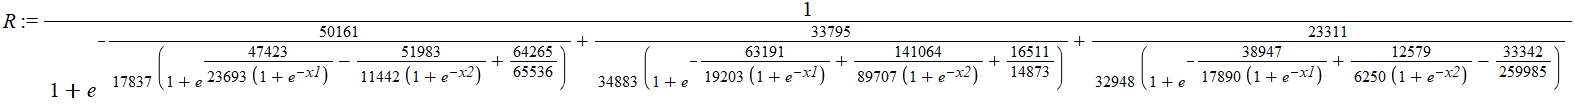
\includegraphics[width=17cm]  {6.png}} 
		\caption{\label{result1} Ranking function $R(x)$}
	\end{figure}
\end{exam}

\section{Experiments}
\label{Experiments}
A prototype of our approach is implemented in Algorithm 4 and we use python to obtain the candidate ranking function $r(u)$ by the package tensorflow\cite{tensorflow2015-whitepaper}, which used in building neural network. All the computations were performed on a PC equipped with a 2.9 GHz Intel Core i5-9400f CPU and 8 GB 2666 MHz DDR4 RAM.
The procedure to synthesize a candidate ranking function for a given loop is embedded in Algorithm 3. In order to facilitate the calculation of $c$, in our experiment, we choose three-layer network structure. The input layer contains $n+1$ neurons when $n$ variables in the loop structure. The hidden layer contains three neurons three neurons and the output layer contains  one neuron. And we set all activation functions as sigmoid function. Moreover, the selection of optimization algorithm, the $\varepsilon $ and ${c_{assume}}$ are set as the tunable parameter in the training.

\subsection{Experimental results}
\label{Experimental results}
Table \ref{loops} shows the loops involved in the experiment. All loops are generated based on two ways: one is from other work, the loops(1,13-14,17) are from \cite{yuan2019ranking}, while loop(18) are from \cite{ben2017multiphase}, and the others like the loops(2-12,15-16,19-25) are gotten by simply make some modifications on the loops which used in the work of \cite{yuan2019ranking} and \cite{ben2017multiphase}. 

And we choose different examples for one-dimension(\romannumeral1:1-6), two-dimensions(\romannumeral2:7-20) and three-dimensions(\romannumeral3:21-25). In addition, the loops with transcendental terms are marked $\bullet$. And the loops without transcendental terms are marked $\circ$. 

\begin{center}
	\captionof{table}{Loops for experiments.($\circ$: loops without transcendental terms; $\bullet$: loops with transcendental terms.)} 
	
	\tablefirsthead{\hline \#& dimension & loop & type \\ \hline  }
	\tablelasttail{\hline}
	
	\tablehead{\hline\multicolumn{4}{|c|}
		{\small\sl continued from previous page}\\\hline
		\#& dimension & loop & type \\   }
	\tabletail{\hline\multicolumn{4}{|c|}{\small\sl continued on next page}\\\hline}
	\begin{supertabular}[H]{|c|c|p{12cm}|c|}{\label{loops}}		
		1 & \romannumeral1 & $while\,x \ge 1,x \le 3\quad do\,x' = 5x - {x^2}$ & $\circ$ \\ \hline  
		2 & \romannumeral1 & $while\,x > 4\quad do\,x' =  - 2x + {\rm{4}}$ & $\circ$ \\ \hline  
		3 & \romannumeral1 & $while\,x > 1\quad do\,x' =  -x$ & $\circ$ \\ \hline 
		4 & \romannumeral1 & $while\,{x^2}{\rm{ - }}3x + 2 \le 0\quad do\,x' = 5x - {x^2}$ & $\circ$ \\ \hline 
		5 & \romannumeral1 & $while\,\;\sin (x) \ge 0,x \ge 1,x \le 6\quad do\,x' =  - x$ & $\bullet$ \\ \hline 
		6 & \romannumeral1 & $while\;\,\sin (x) \ge 0,x \ge 1,x \le 6\quad do\,x' = x + 1 + \cos {(x)^2}$ & $\bullet$ \\ \hline 
		7 & \romannumeral2 & $while\,\;{x_1} - {x_2} \ge 1,{x_1} + {x_2} \ge 1,{x_1} \le 2\quad do\,{x'_1} = {x_1} - 1,{x'_2} = {x_2} - 1$ & $\circ$ \\ \hline 
		8 & \romannumeral2 & $while\,{x_1} \ge 0,{x_2} - 2{x_1} \ge 1,{x_2} \le 3\quad do\,{x'_1} =  - {x_1}^2 - 4{x_2}^2 + 1,{x'_2} =  - {x_1}{x_2} - 1$ & $\circ$ \\ \hline 
		9 & \romannumeral2 & $while\,{x_1}^2 + {x_2}^2 \le 1,\cos ({x_1}) \ge 0\quad do\,{x'_1} = {x_1}^2 + 1,{x'_2} = {x_2}^2 - 1$ & $\bullet$ \\ \hline 
		10 & \romannumeral2 & $while\,{x_1}^2 + {x_2}^2 \le 1\quad do\,{x'_1} = {x_1} - 1 - \cos ({x_1}),{x'_2} = {x_2} - 1 - \cos ({x_2})$ & $\bullet$ \\ \hline 
		11 & \romannumeral2 & $while\,{x_1}^2 + {x_2}^2 \le 1,\cos ({x_1})  \ge 0\quad do\,{x'_1} = {x_1} - 1 - \sin {({x_1})^2},{x'_2} = {x_2} - 1 - \cos {({x_2})^3}$ & $\bullet$ \\ \hline 
		12 & \romannumeral2 & $while\,{x_1} \ge 1,x_1 \le x_2\quad do\,{x'_1} = \frac{{\rm{1}}}{{{\rm{16}}}}{x_1} + 2 + {e^{ - {x_1}}},{x'_2} = \frac{{\rm{1}}}{{{\rm{16}}}}{x_2} + 1$ & $\bullet$ \\ \hline 
		13 & \romannumeral2 & $while\,{x_1}^2 + {x_2}^2 \le 1\quad do\,{x'_1} = {x_1} - {x_2}^2 + 1,{x'_2} = {x_2} + {x_1}^2 - 1$ & $\circ$ \\ \hline 
		14 & \romannumeral2 & $while\,{x_1} + {x_2} \ge 1,{x_1} \le 3,{x_2}^2 \le 1\quad do\,{x'_1} = 5x_1-x_{1}^2,{x'_2} = {x_2}^2 + {x_2}$ & $\circ$ \\ \hline 
		15 & \romannumeral2 & $while\,{x_1}^2 \le 1, {x_2}^2 \le 1\quad do\,{x'_1} = {x_1} + {x_2},{x'_2} = {x_2} - 1$ &$\circ$ \\ \hline 
		16 & \romannumeral2 & $while\,{x_2}^2 - {x_2} + 1 \le {x_1}\quad do\,{x'_1} = -x_1,{x'_2} =  - {x_2}$ & $\circ$ \\ \hline 
		17 & \romannumeral2 & $while\,{x_1} \ge 1,{x_2}^2 + 2{x_1} \le 3{x_2}\quad do\,{x'_1} = 1 + \frac{1}{{{x_1}^2}},{x'_2} =  - {x_1}{x_2} - 3{x_2} + {x_2}^2 + 1$ & $\circ$ \\ \hline 
		18 & \romannumeral2 & $while\,{x_1} > 0,{x_1} \le {x_2}\quad do\,{x'_1} = 2{x_1},{x'_2} = {x_2} + 1$ & $\circ$ \\ \hline 
		19 & \romannumeral2 & $while\,x_1 \ge 1, x_1 \le x_2 \quad do\,{x'_1} = {x_1} + {x_2},{x'_2} = -x_2$ & $\circ$ \\ \hline 
		20 & \romannumeral2 & $while\,{x_1} \ge 0,{x_2} \ge 0\quad do\,{x'_1} = {x_1} + {x_2},{x'_2} = {x_2} - 1$ & $\circ$ \\ \hline 
		21 & \romannumeral3 & $while\,{x_2} \ge 0,{x_2} \le {x_1},{x_1} \le 1\quad do\,{x'_1} = {x_1} + 1,{x'_2} = \frac{1}{4}\tan(x_2) + 1,{x'_3} = -{x_3}$ & $\bullet$ \\ \hline 
		22 & \romannumeral3 & $while\,{x_1}^2 + {x_2}^2 + {x_3}^2 \le 1\quad do\,{x'_1} = {x_1} - 1 - \cos ({x_3}),{x'_2} = {x_2} - 1 - \cos ({x_1}),{x'_3} = {x_3} - 1 - \sin ({x_3})$ & $\bullet$ \\ \hline  
		23 & \romannumeral3 & $while\,{x_1}^2 + {x_2}^2 + {x_3}^2 \le 1,\sin ({x_2}) \ge 0\quad do\,{x'_1} = {x_1} - 1,{x'_2} = {x_2},{x'_3} = \sin {({x_3})^3}$ & $\bullet$ \\ \hline 
		24 & \romannumeral3 & $while\,{x_1}^2 + {x_2}^2 \le 1, x_3 \le 0\quad do\,{x'_1} = \frac{1}{4}{x_1} + \frac{1}{8}{x_2},{x'_2} = \frac{1}{4}{x_1}^2,{x'_3} = \frac{1}{6}{x_3} -1 $ & $\circ$ \\ \hline 
		25 & \romannumeral3 & $while\,{x_2} \ge 1,{x_2} \le {x_1},{x_3} \ge 0\quad do\,{x'_1} = -{x_1},{x'_2} = {x_2},{x'_3} = {x_3} + 1$ & $\circ$ \\
	\end{supertabular}
\end{center}

Table \ref{experiment results} depicted the tunable parameters in the experiment and the weights. The first column in the table denotes the loops from Table \ref{loops}. The next four columns denote all experimental tunable parameters mentioned before. The fifth column denotes the weights obtained by Algorithm 3. The last column denotes the upper bound $c$.

As can be seen from the experimental results in Table \ref{experiment results}, by our verification method states in Section \ref{Verification Process}, the verification of candidate ranking function is no longer limited by the verification tools such as \emph{Z3}. Especially for the loop contains transcendental terms, such as one-dimensional (5-6), two-dimensional (9-12) or three-dimensional (21-23), one may detect their ranking functions by our DNN-based method. In particular, For loop (18), existing methods can only find their multi-phase linear ranking functions. However, we can get a candidate ranking function.

\begin{center}
	\captionof{table}{The tunable parameters and experimental results} 
	\tablefirsthead{\hline loop & ${c_{assume}}$ & $\varepsilon $ & $d$ & optimization 
		
		algorithm &$weight$ & $c$ \\ \hline  }
	\tablelasttail{\hline}
	
	\tablehead{\hline\multicolumn{7}{|c|}
		{\sl continued from previous page}\\\hline
		loop & ${c_{assume}}$ & $\varepsilon $ & $d$ & optimization
		algorithm &$weight$ & $c$ \\   }
	\tabletail{\hline\multicolumn{7}{|c|}{\small\sl continued on next page}\\\hline}
	
	\scriptsize
	\begin{supertabular}[H]{|c|c|c|c|c|p{8.1cm}|c|}\label{experiment results} 		
		
		1 & 50 & 0.05 & 0.001 & ADAM & 
		[[ -5.855921745300293   -2.330543041229248 ]
		
		[-20.364992141723633   18.527238845825195 ]
		
		[ -6.136241912841797   -1.1225796937942505]]
		
		[[1.4383845329284668 1.3277370929718018 0.7966102957725525]]
		& 10.09 \\ \hline
		2 & 50 & 0.05 & 0.001 & ADAM & 
		[[ 1.0260323286056519  2.6372127532958984]
		
		[ 2.592477560043335  -0.6153714060783386]
		
		[ 0.594828188419342  -2.5261006355285645]]
		
		[[-0.5611265301704407 2.0623490810394287 -1.0028291940689087]]
		& 1.23 \\ \hline
		3 & 10 & 0.01 & 0.001 & ADAM & 
		[[-2.3436334133148193 -0.016625851392746 ]
		
		[-0.056898158043623  -1.8876415491104126]
		
		[ 4.553391933441162  -1.6753664016723633]]
		
		[[ 1.128777265548706   2.5279500484466553 -0.9741539359092712]]
		& 0.98 \\ \hline
		4 & 10 & 0.01 & 0.001 & ADAM & 
		[[-2.920186996459961   1.7360831499099731]
		
		[-5.163623809814453   4.203181743621826 ]
		
		[ 1.6039228439331055 -0.1343504935503006]]
		
		[[ 1.128777265548706   2.5279500484466553 -0.9741539359092712]]
		& 4.47 \\ \hline
		5 & 10 & 0.01 & 0.001 & ADADELTA & 
		[[ 1.8124676942825317  1.1652917861938477]
		
		[-2.872796058654785   0.2472831457853317]
		
		[-0.2946441173553467 -1.7745099067687988]]
		
		[[ 1.497663974761963  -2.4328577518463135 -0.796199381351471 ]]
		& 1.25 \\ \hline
		6 & 10 & 0.01 & 0.001 & ADAM &
		[[-2.45465350151062   -3.5235118865966797]
		
		[-3.573195219039917  -1.7213060855865479]
		
		[-9.615031242370605   6.443149089813232 ]]
		
		[[0.2788458168506622 0.4986115992069244 4.53493070602417]]
		& 8.64 \\ \hline
		7 & 2.5 & 0.01 & 0.002 & ADAM & 
		[[-0.9724711775779724 -1.790913701057434 0.1311937719583511]
		
		[-0.4343473315238953 3.5478222370147705 -0.9729806184768677]
		
		[-2.210174798965454 -0.0758214443922043 -2.24971866607666]]
		
		[[-1.6925342082977295  1.333398461341858  -0.1803609728813171]]
		& 1.51 \\ \hline
		8 & 12.5 & 0.05 & 0.002 & ADAM & [[ 1.3154786825180054  0.4052276909351349  0.1627338230609894]
		
		[-0.0130754858255386  0.5321783423423767 -0.3574274182319641]
		
		[ 1.377364993095398   0.1813266575336456  1.0136044025421143]]
		
		[[ 2.0278115272521973 -0.3657838702201843  0.3367987871170044]]
		& 5.56 \\ \hline
		9  & 12.5 & 0.05 & 0.002 & ADAM & [[ 2.7846662998199463 -2.4136955738067627 -1.3070461750030518]
		
		[-4.715053081512451   2.150216579437256   2.7339258193969727]
		
		[-2.258000135421753   1.4488911628723145  0.3058335483074188]]
		
		[[-2.8017733097076416  2.469788074493408  -0.5276959538459778]]
		& 6.28 \\ \hline
		10  & 12.5 & 0.05 & 0.002 & ADAM & [[ 3.03637433052063    4.8203911781311035 -2.6361677646636963]
		
		[-2.137758255004883   0.5550006031990051 -0.438726007938385 ]
		
		[-1.7149194478988647 -1.5624099969863892 -1.8290647268295288]]
		
		[[ 1.4087376594543457 -0.779438316822052  -1.5182971954345703]]
		& 3.67 \\ \hline
		11  & 12.5 & 0.05 & 0.002 & ADAM & [[ 2.6632120609283447  2.6698906421661377 -1.0566554069519043]
		
		[-1.171133279800415  -1.5838327407836914 -1.721509337425232 ]
		
		[-1.7054489850997925 -2.4077670574188232  0.358491837978363 ]]
		
		[[ 1.700181484222412  -0.7515915632247925 -3.1739611625671387]]
		& 5.68 \\ \hline
		12 & 2.5 & 0.01 & 0.002 & ADAM & [[ 0.3941701352596283 -2.3517730236053467  0.2161412388086319]
		
		[ 0.8995246887207031 -2.7943689823150635  0.6710333824157715]
		
		[-2.3223273754119873  1.5255376100540161  1.8248270750045776]]
		
		[[-0.5101912617683411 -2.947547674179077   1.513954520225525 ]]
		& 1.41 \\ \hline
		13 & 12.5 & 0.05 & 0.002 & ADAM & [[-2.0015616416931152  4.5431742668151855 -0.9806060791015625]
		
		[ 3.2906837463378906 -1.5724971294403076 -1.1101324558258057]
		
		[ 2.1770262718200684 -2.0126399993896484  0.1282458603382111]]
		
		[[ 2.812188148498535  -0.9688100218772888 -0.7075088024139404]]
		& 7.88 \\ \hline
		14 & 12.5 & 0.05 & 0.002 & ADAM & [[ 3.6623892784118652 -1.410606861114502  -0.6618162989616394]
		
		[-3.011399745941162   0.7222720384597778  0.8571652770042419]
		
		[12.188863754272461  -3.7000672817230225 -3.3904097080230713]]
		
		[[ 0.3377119898796082 -1.1197441816329956  1.1122510433197021]]
		& 3.90 \\ \hline
		15 & 12.5 & 0.05 & 0.002 & ADAM &  [[-1.8072351217269897  5.725420951843262  -1.3815851211547852]
		
		[ 0.3504117131233215 -3.3405511379241943 -0.0264695025980473]
		
		[-2.0926411151885986 -2.5694515705108643 -3.046679973602295 ]]
		
		[[ 1.9843451976776123 -2.579214572906494  -0.310302734375    ]]
		& 5.07 \\ \hline
		16 & 12.5 & 0.05 & 0.002 & ADAM & [[ 2.5586698055267334  0.4331809282302856 -1.5553065538406372]
		
		[-0.8438130021095276 -0.5035918354988098 -1.6053627729415894]
		
		[-0.5477704405784607 -0.9439965486526489 -0.1063966006040573]]
		
		[[ 0.8558939695358276 -0.3794965744018555 -0.3961026072502136]]
		& 0.46 \\ \hline
		17 & 12.5 & 0.05 & 0.002 & ADAM & [[-0.3921792209148407  3.1874005794525146 -0.865526020526886 ]
		
		[ 2.1137895584106445 -1.799368977546692  -0.703197181224823 ]
		
		[-0.5424444079399109  4.590944290161133  -1.416419506072998 ]]
		
		[[ 0.6584115028381348 -1.321570634841919   1.2126175165176392]]
		& 6.66 \\ \hline
		18 & 0.5 & 0.001 & 0.001 & ADADELTA & [[ 1.048069953918457   2.0997307300567627 -2.3266866207122803]
		
		[ 3.4703633785247803 -0.5784722566604614 -2.340416431427002 ]
		
		[-1.4391871690750122 -1.5317275524139404  2.1755189895629883]]
		
		[[-0.760312020778656  -1.1201003789901733  1.9844242334365845]]
		& 0.48 \\ \hline
		19 & 12.5 & 0.05 & 0.002 & ADAM & [[-2.507380723953247  -0.1853876709938049 -2.0108020305633545]
		
		[-0.083501785993576  -2.4635047912597656  0.7140545845031738]
		
		[-0.3050325810909271  3.7262420654296875 -1.5262598991394043]]
		
		[[-0.5840973258018494 -1.3084328174591064  1.5039777755737305]]
		& 1.93 \\ \hline
		20 & 2.5 & 0.01 & 0.002 & ADAM & [[2.3963534832000732 3.0890965461730957 -0.8048329949378967]
		
		[-2.9532835483551025 4.063777923583984 -2.323068141937256]
		
		[-2.499047040939331 3.341022491455078 2.2167253494262695]]
		
		[0.4436832368373871 0.8593196868896484 0.7724987268447876]
		& 0.88 \\ \hline
		21 & 20/3 & 0.1 & 0.005 & ADAM & 
		[[-2.174838066101074  -0.6407662034034729 -1.170314908027649 1.511257290840149 ]
		[-0.3066220283508301  2.0138161182403564  0.490244060754776
		1.3864461183547974]
		[-2.763887882232666  -3.4592125415802     0.1967869102954865
		3.6580541133880615]]
		[[ 0.8110175132751465 -1.3365472555160522  3.5431087017059326]]
		& 3.59 \\ \hline
		22 & 20/3 & 0.1 & 0.005 & ADAM &  [[ 2.1336159706115723  1.1494638919830322  1.5633387565612793
		-0.6107999682426453]
		[-1.323683500289917  -1.2304725646972656 -1.2066571712493896
		-0.3168062269687653]
		[-1.8960381746292114 -3.18878436088562   -0.0216311700642109
		0.9264867901802063]]
		[[ 1.537946343421936  -1.1959309577941895 -1.6288409233093262]]
		& 5.93 \\ \hline
		23 & 20/3 & 0.1 & 0.005 & ADADELTA & [[ 9.287436485290527  -0.319311797618866  -1.9479351043701172
		-2.3329615592956543]
		[-2.340475082397461  -2.9602091312408447 -3.5425498485565186
		-2.3635144233703613]
		[-3.0034594535827637  0.5185515880584717  0.9227628111839294
		-0.2369051575660706]]
		[[ 1.9518927335739136  0.056944951415062  -2.5973238945007324]]
		& 5.01 \\ \hline
		24 & 20/3 & 0.1 & 0.005 & ADAM & [[ 2.5731589794158936 -1.297593116760254  -3.3742153644561768
		-0.3204583525657654]
		[ 2.260584592819214  -3.5005502700805664  0.7450693845748901
		-0.8528845906257629]
		[-2.1284077167510986  4.673758029937744   0.0090981414541602
		-0.0352618470788002]]
		[[-0.6772419214248657 -2.3815860748291016  2.3263206481933594]]
		& 4.89 \\ \hline
		25 & 20/3 & 0.1 & 0.005 & ADAM &[[ 3.2802696228027344  0.0690874233841896 -0.435204029083252
		-2.0471887588500977]
		[-2.0195391178131104 -0.7831394672393799  1.593719482421875
		-0.6381518244743347]
		[ 1.090225338935852  -1.6407567262649536 -0.3074676394462585
		-1.6080644130706787]]
		[[ 2.244703769683838  -1.851402759552002  -0.3808052837848663]]
		& 2.21 \\ 
	\end{supertabular}
\end{center}
Note that the ${n_1}$ and ${n_2}$ in Algorithm 2 also is the tunable parameter in the experiment, but in most of the next experiments, let ${n_1}  = 0.5$ ${n_2} = 0.2$. However, for loop (18), we will adjust the ${n_1} = 0.5$ and ${n_2} = 0.3$ to achieve the best training effect.

\subsection{Method Comparsion}
\label{Method Comparsion}
Most of existing methods focus on the synthesis of polynomial ranking functions, but not all terminating loops have polynomial ranking functions. According to the universal approximation theorem, our method can detect more expressive ranking functions by DNN, which is non-polynomial. Moreover, compared with SVM-basedmethod, we propose a new method to check if a candidate ranking function is exact a ranking function. Different from existing method depends on \emph{Z3}, our method can verify if a candidate ranking function with transcendental terms is exact a ranking function.

We next compared our DNN-based method with QE-based method\cite{chen2007discovering}, SVM-based method \cite{yuan2019ranking} and method for multi-phase linear ranking functions in \cite{ben2017multiphase}.

\textbf{\emph{A.}} For QE-based method\cite{chen2007discovering}, QE-based method can only deal with the polynomial loops and synthesis polynomial ranking functions. But our method can not only deal with the polynomial loops, but also the loops with transcendental terms. Moreover, the ranking functions obtained by our method are non-polynomial.

\textbf{\emph{B.}} For SVM-based method\cite{yuan2019ranking}, it is main idea is: Firstly, for a given loop, the synthesis of polynomial ranking functions of this loop is reduced to the classfication problem; Secondly, a candidate ranking function is obtained by SVM; Finally, the SMT tool \emph{Z3} is used to check if the obtained candidate ranking function is exact a ranking function. Therefore, the SVM-based methods rely heavily on \emph{Z3}. However, \emph{Z3} cannot deal with the expressions with transcendental terms such as $\sin( \cdot )$ and $\cos(\cdot)$. Thus, the SVM-based method cannot deal with the loops (5-6,9-12,21-23) with transcendental terms. However, by Proposition 1 and its Remark, for the loops with transcendental terms, we propose a new approach to check if a candidate ranking function is exact a ranking function.

\textbf{\emph{C.}} \cite{ben2017multiphase} presents an LP-based method to synthesize multi-phase linear ranking functions for single- path linear-constraints loops. For loop (18) having multi-phase ranking functions by \cite{ben2017multiphase}, our method indeed can find its global ranking functions by DNN. One of the reasons is, we think, the neural network can approximate any function under given conditions according to the universal approximation theorem. Therefore, the multi-phase ranking functions of loop (18) may be approximated by the DNN. We illustrate this by following example.
\begin{exam}\label{exm7}
	Consider the following loop:
	
	$$\begin{array}{l}
	while\,{x_1} > 0,{x_1} \le {x_2}\quad do\,\\
	{{x_1}'} = 2{x_1},{{x_2}'} = {x_2} + 1
	\end{array}$$
	
	Firstly, we choose the neural network structure, as follows:
	\begin{figure}[H] 
		\center{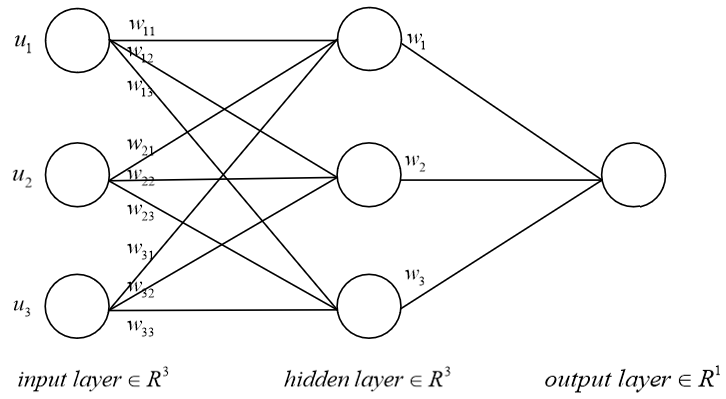
\includegraphics[width=10cm]  {7.png}} 
		\caption{}
		\label{neural structure for 3 neurons}
	\end{figure}
	Secondly, we assume that ${c_{assume}} = 0.50$ and set $\varepsilon  = 0.001$. Thus we can calculate the step $d = \frac{\varepsilon }{{n\cdot{c_{assume}}}} = \frac{{0.001}}{{a2\cdot0.50}} = 0.001$ and construct $N_{sample}$ by Algorithm 1. Thirdly, we construct the train-set $D_{train}$ by Algorithm 2. It should be noted that we set ${n_1}$ to 0.5 and set ${n_2}$ to 0.3 in Algorithm 2.
	
	We begin to adjust parameters and make a training until the accuracy of test-set is 1. We find that when we choose ADAM as optimization algorithm and set learning rate to 0.1, the accuracy of test-set reaches 1.
	
	By Algorithm 3, we get
	
	\begin{table}[H]
		\begin{center}
			\setlength{\abovecaptionskip}{0pt}   
			\setlength{\belowcaptionskip}{0pt}
			\caption{Output weights}
			\begin{tabular}{|c|lll|}
				\hline
				\multirow{3}{*}{the weights $w_{ji}$:} & 1.048069953918457 & 2.0997307300567627   & -2.3266866207122803   \\
				& 3.4703633785247803  & -0.5784722566604614   & -2.340416431427002   \\
				& -1.4391871690750122 & -1.5317275524139404 & 2.1755189895629883 \\
				\hline the weights $w_{i}$:&-0.760312020778656   & -1.1201003789901733 & 1.9844242334365845 \\ \hline
			\end{tabular}
		\end{center}
	\end{table}
	
	By Table 6, Since $w_{ji}$ and $w_i$ are known, we can get a candidate ranking function $r(u)$. By method for computing $c$ states in Section \ref{Computation}, for the candidate ranking function $r(u)$, we get $c = 0.48 < 0.50 = {c_{assume}}$.
	
	Therefore, by Proposition 1 and its Remark, $r(u)$ is the ranking function over $U(\Omega )$. By Theorem \ref{thm1}, we can get the desired ranking function $R(x)$ over $\Omega $ of loop (18), as follows:
	
	\begin{figure}[H] 
		\center{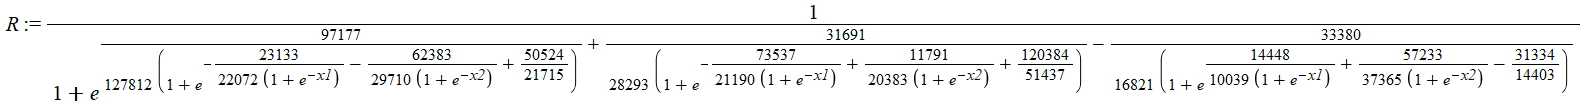
\includegraphics[width=17cm]  {8.png}} 
		\caption{\label{result2} Ranking function $R(x)$}
	\end{figure}
\end{exam}

\section{Conclusion}
\label{Conclusion}
In this paper, we propose a DNN-based method to synthesize non-polynomial ranking functions for loop programs. We leverage DNN to construct a candidate ranking function first, and then use the method states in Section \ref{Verification Process}, which states that if $c<c_{assume}$ holds, to verify if the candidate ranking function by DNN is exact a ranking function of the loop program. Compared with existing methods, our methods can deal with loops with transcendental terms and detect more expressive ranking functions. What's more, for some loops having multi-phase ranking functions, our method can also find their global ranking functions. However, our method still has its own limitations. For instance, when a candidate ranking function $r(u)$ is obtained by DNN, in order to verify check if $r(u)$ is a ranking function, we need to compare the upper bound $c$ of $\left| {\bigtriangledown (r(u) - r(u'))} \right|$ with $c_{assume}$. In Section \ref{Computation}, by (\ref{equ:|r(u)/u_k|}), (\ref{equ:|r(u')/u_k|}) and (\ref{equ:method(u)}), we know that the computation of the upper bound $c$  depends on the upper bound of ${\left| {\frac{{\partial (m \circ {f_j} \circ {U^{ - 1}}(u))}}{{\partial {u_k}}}} \right|}$. But there is no general method to compute the upper bound of ${\left| {\frac{{\partial (m \circ {f_j} \circ {U^{ - 1}}(u))}}{{\partial {u_k}}}} \right|}$. If the upper bound of ${\left| {\frac{{\partial (m \circ {f_j} \circ {U^{ - 1}}(u))}}{{\partial {u_k}}}} \right|}$ cannot be obtained, our method fails. In addition, if $c<c_{assume}$ does not hold, we have to increase the value of $c_{assume}$ to get a new $c^{(1)}_{assume}$. Then we invoke Algorithm 3 to get another candidate $r^{(1)}(u)$ and compute the value of $c^{(1)}$ to compare $c^{(1)}$ with $c^{(1)}_{assume}$. If $c^{(1)}<c^{(1)}_{assume}$ holds, then $r^{(1)}(u)$ is desire a ranking function over $U(\Omega)$. If not, the above process have to proceed.


\begin{acknowledgements}
This research is partially supported by the National Natural Science Foundation of China NNSFC(61572024,
11771421,61103110),the Natural Science Foundation of Chongqing (cstc2019jcyj-msxmX0638) and Chinese Academy of Sciences ``Light of West China" program.
\end{acknowledgements}


% Authors must disclose all relationships or interests that 
% could have direct or potential influence or impart bias on 
% the work: 
%
\section*{Conflict of interest}
The authors declare that no support, financial or otherwise, has been received from any organization that may have an interest in the submitted work and there are no other relationships or activities that could appear to have influenced the submitted work.

% The authors declare that they have no conflict of interest.


% BibTeX users please use one of
\bibliographystyle{spbasic}      % basic style, author-year citations
%\bibliographystyle{spmpsci}      % mathematics and physical sciences
%\bibliographystyle{spphys}       % APS-like style for physics
\bibliography{mybibfile}   % name your BibTeX data base

% Non-BibTeX users please use
%\begin{thebibliography}{}
%
% and use \bibitem to create references. Consult the Instructions
% for authors for reference list style.
%
%\bibitem{RefJ}
% Format for Journal Reference
%Author, Article title, Journal, Volume, page numbers (year)
% Format for books
%\bibitem{RefB}
%Author, Book title, page numbers. Publisher, place (year)
% etc
%\end{thebibliography}

\end{document}
% end of file template.tex

